\documentclass[journal,twoside,web]{ieeecolor}
\usepackage{generic}
\pdfminorversion=4

\let\proof\relax
\let\endproof\relax
\usepackage{amsthm}
\usepackage{graphicx}
\usepackage{epsfig}
\usepackage{times}
\usepackage{amsmath}
\usepackage{amssymb}
\usepackage{cleveref}
\usepackage{subcaption,graphicx}
\usepackage{mathtools, cuted}
\usepackage{todonotes}
\usepackage{url}
\usepackage{color}
\usepackage{mathrsfs}
\usepackage{multirow}
\usepackage{caption}
\usepackage{subcaption}
\usepackage{cite}
\usepackage{wrapfig}
\usepackage{float}
\usepackage{mleftright}
\usepackage{nth}
\usepackage{dsfont}
\usepackage[normalem]{ulem}
\usepackage{tikz}
\usetikzlibrary{shapes,arrows}

\newtheorem{theorem}{Theorem}
\newtheorem{acknowledgement}[theorem]{Acknowledgement}
\newtheorem{algorithm}[theorem]{Algorithm}
\newtheorem{axiom}[theorem]{Axiom}
\newtheorem{assumption}[theorem]{Assumption}
\newtheorem{properties}[theorem]{Properties}
\newtheorem{case}[theorem]{Case}
\newtheorem{claim}[theorem]{Claim}
\newtheorem{conclusion}[theorem]{Conclusion}
\newtheorem{condition}[theorem]{Condition}
\newtheorem{conjecture}[theorem]{Conjecture}
\newtheorem{corollary}{Corollary}
\newtheorem{criterion}[theorem]{Criterion}
\newtheorem{con}[theorem]{Condition}
\newtheorem{definition}{Definition}
\newtheorem{exercise}[theorem]{Exercise}
\newtheorem{lemma}{Lemma}
\newtheorem{notation}[theorem]{Notation}
\newtheorem{problem}[theorem]{Problem}
\newtheorem{proposition}[theorem]{Proposition}
\newtheorem{solution}[theorem]{Solution}
\newtheorem{summary}[theorem]{Summary}
\newtheorem{remark}{Remark}
\newtheorem{example}[theorem]{Example}
\newtheorem{thm}{Theorem}
\newtheorem{cor}{Corollary}
\newtheorem{lem}{Lemma}
\newtheorem{prop}{Proposition}
\newtheorem{defn}{Definition}
\newtheorem{rem}{Remark}
\newtheorem{ass}{Assumption}

\DeclareMathOperator*{\infm}{inf}
\DeclareMathOperator*{\minimize}{minimize}
\DeclareMathOperator*{\maximize}{maximize}
\DeclareMathOperator*{\subjt}{subject \ to}
\DeclareMathOperator*{\sgn}{sign}
\DeclareMathOperator*{\argmin}{argmin}
\newcommand{\argmax}[1]{\underset{#1}{\operatorname{arg}\,\operatorname{max}}\;}
\newcommand{\pe}{\psi}
\newcommand{\R}{\mathbb{R}}
\newcommand{\trace}{\text{tr}}
\newcommand{\vecu}{{\bf u}}
\newcommand{\vece}{{\bf e}}
\newcommand{\vecc}{{\bf c}}
\newcommand{\dom}{\cal{D}}
\newcommand{\op}{\cal{L}}
\newcommand{\dop}{\cal{E}}
\newcommand{\x}{\textbf{x}}
\newcommand{\z}{\mathbb{Z}}
\newcommand{\real}{\mathbb{R}}
\newcommand{\p}{\partial}
\newcommand{\ps}{p^{\star}}
\newcommand{\PF}{\mathbb{P}}
\newcommand{\Tyx}{T_{y\rightarrow x}(p)}
\newcommand{\bi}{\begin{itemize}}
\newcommand{\ei}{\end{itemize}}
\newcommand{\bd}{\begin{displaymath}}
\newcommand{\ed}{\end{displaymath}}
\newcommand{\be}{\begin{align*}}
\newcommand{\ee}{\end{align*}}
\newcommand{\si}{\Sigma^{-1}}
\newcommand\norm[1]{\left\lVert#1\right\rVert}
\newcommand{\sub}[2]{(#1)_{(#2)}}

\title{\LARGE \bf Robust Optimization via Continuous-Time Dynamics}

\author{Keivan Ebrahimi, Nicola Elia, and Umesh Vaidya\\
\thanks{Financial support from the National Science Foundation grants CNS-1329915, ECCS-1150405, CIF-1220643, and ECCS-1810079 and from AFOSR grant FA95500119 are gratefully acknowledged. K. Ebrahimi is with the Department of Electrical \& Computer Engineering, Iowa State University, Ames, Iowa. U. Vaidya is with the Department of Mechanical Engineering, Clemson University, Clemson SC.  N. Elia is with the Department of Electrical and Computer Engineering, University of Minnesota, Twin Cities.
{\tt\small keivan@iastate.edu},
{\tt\small uvaidya@clemson.edu},
{\tt\small nelia@umn.edu}
}}

\begin{document}

\pagestyle{headings}
\setcounter{page}{1}
\pagenumbering{arabic}

\maketitle

\begin{abstract}
We propose a dynamical system-based approach for solving robust optimization problems in a general convex-concave framework. Our proposed approach offers a novel solution to robust optimization problems by introducing a continuous-time dynamical system, which we call ${\cal RO}$ dynamics. Unlike the well-known primal-dual gradient dynamics for solving regular optimization problems, our new approach does not rely on the gradient of the Lagrangian function to derive the vector field. In ${\cal RO}$ dynamics, the uncertain variable is treated as a dynamical state, and we demonstrate that the globally asymptotically stable equilibrium point of ${\cal RO}$ dynamics can recover robust optimal solutions for a general class of convex-concave robust optimization problems. This is achieved without any prior knowledge of the formulation of the specific problem. Furthermore, our approach is amenable to decentralized implementation, enabling the dynamics to autonomously derive an unknown system to solve the robust optimization problem by using output feedback only. This is while the existing solutions such as the robust counterpart and scenario-based random sampling assume that the problem formulation is completely known a priori. In contrast, our proposed method is not constrained by these limitations and is suitable for real-time applications in dynamic environments. To demonstrate the effectiveness of our approach, we provide a simulation example of a robust location and placement problem with time-varying anchor locations, among others. Our proposed dynamical system-based approach offers better properties compared to traditional approaches and demonstrates the potential to solve a broad range of robust optimization problems in a decentralized manner.
\end{abstract}

\section{Introduction}

With emerging applications that require solving real-time optimization problems in a reactive manner, this paper describes how interacting dynamical systems can find a robust solution for a broad class of robust optimization problems. This is particularly relevant in situations where physical systems must be steered towards optimal operating conditions, without prior knowledge of the functions to be optimized or the model of the uncertainty affecting the optimization. Specifically, we propose a real-time approach to solving robust optimization problems, which has become increasingly important in recent years \cite{he2022}. Optimization problems often involve various forms of uncertainty in the problem data. Two different approaches can be used: stochastic optimization, where uncertainty is treated as a random variable, or robust optimization (${\cal RO}$), where uncertainty is assumed to be deterministic and bounded. Unlike stochastic optimization, ${\cal RO}$ does not require any known probability distributions in the problem data. Instead, ${\cal RO}$ assumes that the uncertain data reside within a predefined uncertainty set, for which constraint violation cannot be tolerated. For more information on robust and stochastic optimization-based approaches, see \cite{bental2009}, \cite{bertsimas2011}, and the references therein. Early works on ${\cal RO}$ include \cite{soyster1976}, which considered robust linear optimization with ellipsoidal uncertainty sets, and \cite{falk1976}, which presented exact solutions of inexact linear programs as a simple case of ${\cal RO}$.

The problem of robust linear programming was studied in \cite{bental1999}, while robust conic-quadratic optimization and robust semi-definite optimization were discussed in \cite{bental2002} and \cite{bental1998}, respectively. Refer to \cite{bertsimas2011} and \cite{beyer2007} for a survey of different ${\cal RO}$ problem solutions.
\cite{xu2009} and \cite{xu2010} showed that some of the machine learning algorithms such as the norm-regularized support vector machine and the Lasso problem could be interpreted as ${\cal RO}$ problems. In addition to that, several papers focused on making machine learning problems robust against outliers, parameter uncertainties, and data perturbations by techniques such as adversarial training \cite{lanckriet2003, bhattacharyya2004a, bhattacharyya2004b, trafalis2007, namkoong2016, sinha2018, esfandiari2019}.

One of the main standard approaches for solving ${\cal RO}$ problems involves constructing a robust counterpart (RC) equivalent to the ${\cal RO}$ problem \cite{bental2009}. This widely used method essentially tries to find a deterministic equivalent to ${\cal RO}$ problem through a reformulation. In this sense, the practicality of robust programming depends on whether or not its RC is computationally tractable. An overview of different RO problems with tractable conjugates can be found in \cite{gorissen20152} Table 1 for some of which RC cannot be found.
The reformulation approach to solving the ${\cal RO}$ problem, which is often a challenging, albeit usually convex, optimization problem, has the deficiency of suffering from case-by-case scenarios depending on the specific form of the uncertainty constraint and the specific form of the uncertainty set. In other words, depending on how simple the uncertainty set looks and based on the optimization problem type (whether it is linear programming, quadratic programming, second-order cone programming, semi-definite programming, etc.), an RC is being calculated and provided at hand. These reformulations may be computationally more expensive than other approaches \cite{bertsimas2016}. Hence, the absence of a unified framework for solving a general class of ${\cal RO}$ problems without prior knowledge of the problem formulation is strongly felt.

By calculating a concave conjugate of nonlinear constraint functions and supporting the function of uncertainty sets, \cite{bental20152} and \cite{gorissen20152} used the Fenchel duality to obtain a tractable RC for new classes of robust nonlinear optimization (RNO) problems. It may be the case that no closed form is available for the convex conjugate function of an uncertainty set or convex/concave conjugates of a non-linear constraint. In this case, these approaches do not obtain the RC for many sets of nonlinear uncertainties and constraints.

An alternative randomized approach based on constraint sampling is an approximate probabilistic relaxation solution to ${\cal RO}$ problems as seen in \cite{calafiore2004} and \cite{calafiore2010} where a finite set of high-dimensional deterministic optimization problems obtained from sampling are solved. This approach does not require concavity of the constrain in the uncertain variable but due to the large number of required scenarios to approximate the stochasticity of these problems, the stochastic optimization involves formulating a large-scale scenario program, which is in general computationally demanding. To address this issue, \cite{rostampour2021} presented two methods. The first is to decompose the large-scale scenario program into distributed scenario programs using the alternating-direction multiplier method (ADMM). The second method is to use a soft communication scheme to reduce the required communication between the subproblems.

In another effort, \cite{bental2015} incorporated the min-max behavior of ${\cal RO}$ problems to solve them by an oracle-based approximate robust optimization algorithm based on oracle-based subgradient descent and interior point methods. The proposed algorithms find an approximate robust solution using a number of calls to an oracle that solves the original (non-robust) problem. However, the solution would be approximated with some predetermined accuracy, $\eta$, with the number of iterations growing to ${\cal O}(\frac{1}{\eta})$, as the algorithm approximates the RC by invoking the Oracle a polynomial number of times.
In \cite{mutapcic2009}, a cutting-plane algorithm treats ${\cal RO}$ problem as semi-infinite programming and iterates between optimization problem with fixed uncertainties values and posterior worst-case analysis to possibly find the robust solution.
The worst-case analysis depends on finding pessimization oracles that may be exact or approximate. The robust problem cannot be solved by the cutting plane method if the pessimization is approximate, that is, when the worst-case functions are being computed approximately. In another effort, \cite{nguyen2018} tried to alleviate the computational cost of Oracle-based methods by finding the approximate solution for ${\cal RO}$ problem iteratively with first-order oracles.

Robust optimization over time (ROOT) is another line of research in which robust optimization and dynamic optimization (a certain type of optimization to model uncertainties resulting from environmental changes) are combined. In these problems, robust solutions usually do not remain desirable forever and need to be changed after some major environmental change. \cite{yazdani2023} provides a review of ROOT papers that includes a classification of these problems with their respective definitions.

Compared with existing ${\cal RO}$ methods, we point out that most existing algorithms are in a one-shot manner, as they require a priori knowledge of the uncertainty set model in order to even write the optimization problem to be solved. In contrast, our approach is independent of knowledge of the uncertainty set model as long as it is convex and the adversary variables enter concavely in the constraints and cost function. This opens up the possibility of having distributed real-time implementations of such systems in many settings where the uncertainty model and exact knowledge of the cost function and constraints are not available.

In this paper, we provide the architecture of such a dynamical system that converges to the optimal robust solution for a large class of ${\cal RO}$ problems.

Although our approach is inspired by the work on primal-dual systems \cite{arrow1958,feijer2010}, it presents significant architectural and convergence challenges described in the paper. A key technical contribution is finding the right architecture of the dynamical system for which a non-standard Lyapunov function can help to prove global convergence to an optimal ${\cal RO}$ solution. The proposed continuous-time optimization system can solve a general class of ${\cal RO}$ problems where the cost function and the constraints are convex (concave) with respect to the decision variables (uncertain variables) and the uncertainty sets are convex\footnote{Preliminary convergence results for a special formulation appeared without proofs in \cite{ebrahimi2019continuous}. In this paper, we generalize the problem formulation and provide complete proofs, which are the core of our contributions.}. This class includes all the cases in \cite[~Table 1]{gorissen20152}.

The remainder of this paper is organized as follows. In Section \ref{sec_RO}, we present the problem statement of ${\cal RO}$ in a slightly generalized form. In Section \ref{section_saddle}, the characterization of saddle property and KKT optimality conditions along with the Lagrangian function for ${\cal RO}$ problem are provided. The main results on how to construct the ${\cal RO}$ dynamics is presented in Section \ref{section_pddynamics}. This section also includes the Lyapunov-based global convergence result. We then present simulation results in Section \ref{section_simulations} followed by conclusions in Section \ref{section_conclusions}.
Finally, detailed proofs are mentioned in the Appendix.

\section{Notations}\label{notations}

We define $i=0,\cdots,N$ as $i_{[N]}$, and $i=1,\cdots,N$ as $i^+_{[N]}$. In addition, $\left[\cdot\right]_\eta^+$ shows the positive projection defined as follows for the scalar-valued function $P$
\begin{align} \label{proj}
[P]_\eta^+:=\left\{\begin{array}{ccl}P&{\rm if}& P>0 \;{\rm or} \;\eta>0\\
0&{\rm otherwise}
\end{array}\right..
\end{align}
For vector-valued $P$, the projection is defined element-wise.

\section{Robust Optimization Problems}\label{sec_RO}
Given an objective $f_0(x)$ to optimize, subject to constraints $f_i(x,u_i) \leq 0$ with uncertain parameters, $\{u_i\}$, a classical robust optimization problem has the following form
$$
\begin{array}{ccc}
\mu&:=&\underset{x}{\min}\; f_0(x)\\
&&\text{s.t.}\;\;\;f_i(x,u_i)\leq 0,\;\;\;\; \forall \,u_i\in {\cal U}_i,\;\;\;i^+_{[N]}.
\end{array}
$$
where $x\in \real^n$ is a vector of decision variables, $f_0$ and $f_i$ are $\real^n \to \real$ functions, and the uncertainty parameters $u_i \in \real^{m_i}$ are assumed to take arbitrary values in certain convex compact uncertainty sets ${\cal U}_i \subseteq \real^{m_i}$.
The above problem is typically a semi-infinite optimization due to the cardinality of the ${\cal U}_i$. However, each robust constraint can be rewritten as a maximization problem as\footnote{Since the uncertainty set is compact,
the supremum is attained within the set; therefore, we can replace "sup" with "max" in our formulation.}
\begin{align}
\begin{array}{ccc}
\mu&:=&\underset{x}{\min}\; f_0(x)\\
&&\text{s.t.}\;\;\;\displaystyle\max_{{u_i\in \cal U}_i} f_i(x,u_i)\leq 0,\;\;\;\;i^+_{[N]}
\end{array}\;.\label{standardRO}
\end{align}

We consider a slight variation of (\ref{standardRO}), which takes the following under the assumptions stated below.
\begin{equation}\label{RO0}
\mathcal{RO}_0\left\{ \begin{array}{ccc}
&\mu:=\underset{x}{\min} \;\underset{u_0\in {\cal U}_0}{\max}\; f_0(x,u_0)\\
&\text{s.t.}\;\;\;\underset{u_i\in {\cal U}_i}{\max}\;\; f_i(x,u_i)\leq 0\;,\;i^+_{[N]},\\ \\
&{\cal U}_i:=\{u_ i\in \mathbb{R}^{m_i}\;:\;h_{ij}(u_i)\leq 0,\;\;j_{[K_i]}\}\;,\;i_{[N]}
\end{array}\right.
\end{equation}
The problem in (\ref{RO0}) reduces to the one in (\ref{standardRO}) when ${\cal U}_0$ is a singleton.
Following \cite{bental2009-2} and without loss of generality, we consider the ${\cal RO}$ problem dealing with constraint-wise uncertainties where each constraint $f_i$ is only a function of $u_i$.
The functions $f_i$ and $h_{ij}$ have scalar values with the following assumptions.

\begin{assumption}\label{assume1} The functions $h_{ij}(u_i)$ are convex in $u_i$ for $i_{[N]}$ and $j^+_{[K_i]}$.
The function $f_0(x,u_0)$ is strictly convex in $x$ for any $u_0\in {\cal U}_0$, and concave in $u_0$ for any $x$. Also, for $i^+_{[N]}$, $f_i(x,u_i)$ is convex in $x$ for fixed $u_i$ and concave in $u_i\in {\cal U}_i$, for fixed $x$.
Finally, the functions $f_i$ and $h_i$ $i_{[N]}$ are $C^1$ with local Lipschitz gradients.
\end{assumption}

\begin{assumption} \label{assume_feasible} Existence of optimal solutions and strong duality.

\begin{enumerate}
\item [A1] ${\cal RO}$ problem (\ref{RO}) is feasible. An optimal min-max solution $(x^\star,u^\star)$ exists and $\mu$ in the ${\cal RO}$ problem (\ref{RO}) is finite.
\item [A2] ${\cal RO}$ problem satisfies the Slater constraint qualification, for both the upper level optimization (\ref{RO2}) and the lower level (\ref{G.eq})
 \cite{bental2009-2}, that is,
for all $i_{[N]}$ and all $j^+_{[K_i]}$, there exist $u_i \in {\cal U}_i$ such that $h_{ij}(u_i)<0,\;$  and
for $i^+_{[N]}$,  there exists $x \in \mathbb{R}^n$ such that, ${\cal F}_i(x)<0$\;.
\end{enumerate}
\end{assumption}
\begin{remark}
    It should be noted that the uncertainty is often parametrized affinely in ${\cal RO}$ problem; hence, the concavity property of the $f_i$ functions is automatically satisfied.
\end{remark}
\begin{remark} \label{strong_duality_rem}
Assumption [A2] guarantees that ${\cal RO}$ problem enjoys strong duality for upper and lower level optimization problems (\ref{RO2}) and (\ref{G.eq}) \cite[Section~5.2.3, 5.9.1]{boyd2004}. Moreover, it enforces that saddle point and optimal dual solutions exist \cite{bental2009-2}. For conditions less restrictive than those of Slater, the interested reader may refer to \cite{jeyakumar2010}.
\end{remark}

Finally, we introduce the problem we consider in the paper, a slight generalization of ${\cal RO}_0$ in (\ref{RO0}).
\begin{equation}{\cal RO}\left\{\begin{array}{ccc}
&\mu:=\underset{x}{\min} \;\underset{u_0\in {\cal U}_0}{\max}\; f_0(x,u_0)+\displaystyle\sum_{i=1}^N c_i \underset{u_i\in {\cal U}_i}{\max}\;\; f_i(x,u_i)\label{RO}\\ \\
&\text{s.t.}\;\;\;\underset{u_i\in {\cal U}_i}{\max}\;\; f_i(x,u_i)\leq 0\;,\;i^+_{[N]},\\ \\
&{\cal U}_i:=\{u_ i\in \mathbb{R}^{m_i}\;:\;h_{ij}(u_i)\leq 0,\;\;j_{[K_i]}\}\;,\;i_{[N]}
\end{array}\right.
\end{equation}
where $c_i\geq 0$ for $i^+_{[N]}$. This setting can be seen as an elementary regularized version of more common formulations ${\cal RO}_0$ obtained for $c_i=0$, $i_{[N]}^+$.
The role of $c_i$ is further clarified in Remark \ref{active_inactive_constraint_rem}.

It is convenient to rewrite ${\cal RO}$ in the following form
\begin{align}
&\mu:=\underset{x}{\min} \; {\cal F}_0(x)+\sum_{i=1}^N c_i{\cal F}_i(x)\label{RO2}\\
&\;\;\text{s.t.}\;\;\;{\cal F}_i(x)\leq 0\;,\;i^+_{[N]}\;,\nonumber
\end{align}
where
\begin{equation}\label{G.eq}
{\cal F}_i(x):=\max_{u_i\in {\cal U}_i} f_i(x,u_i)\;,\; i_{[N]}\;.
\end{equation}
In this paper, we often call (\ref{G.eq}) as the "lower optimization problems", and the minimization in (\ref{RO2}) as the "upper optimization".

 As already mentioned, our formulation includes the typical robust optimization formulation ${\cal RO}_0$
\begin{equation}
\begin{array}{lcc}
\mu=&\;\displaystyle\min_x f_0(x)\\
s.t.&\; {\cal F}_i(x)\leq 0,\;\;i^+_{[N]}
\end{array}\;,
\label{RO3}
\end{equation}
or the form below that is popular in the machine learning context \cite{rafique2022,zhang2021}
\begin{equation}
\mu=\;\displaystyle\min_x\max_{u\in {\cal U}} f_0(x,u)\;.
\end{equation}
We finally introduce the following assumption valid for most of the paper.

\begin{assumption} \label{assume_c>0}
\begin{enumerate}
\item [A3] $c_i > 0$ for $i^+_{[N]}$.
\end{enumerate}
\end{assumption}

\begin{remark} \label{active_inactive_constraint_rem}
The assumption [A3] is made for technical reasons to simplify and streamline the derivations. It is used to impose arbitrarily small regularization terms in order to provide convergence proof in the event that some of the robust constraints are inactive. On the other hand, if a constraint is active, the corresponding $c_i$s can be zero. So, all $c_i$s can be equal to zero under the classical but stronger assumption that all the robust constraints are active.
\end{remark}

\subsection{Robust feasible solution and robust counterpart}
A meaningful solution to ${\cal RO}$ problem (\ref{RO}) has to be immune against the uncertainties in the sense that the solution vector $x$ should satisfy the constraints for all $u_i$'s within the uncertainty sets\footnote{Similar to what is meant by feasibility in Robust Control \cite{zhou1995}.}. Such vector $x$ is called a robust feasible solution (RFS). One approach to solving the problem (\ref{RO}) is to try to compute (\ref{G.eq}) in closed form.

For various important combinations of constraint functions $f_i$ and uncertainty sets ${\cal U}_i$, ($i>0$) it is possible to obtain an explicit convex function ${\cal F}_i$ \cite{bental2009}. A classical example is when $f_i$ is linear in $x$ for fixed $u_i$ and linear in $u_i$ for fixed $x$, while ${\cal U}_i$ is an ellipsoidal set.
Then, ${\cal F}_i$ can be easily derived as an explicit second-order conic function.
In this case, ${\cal RO}$ problem (\ref{RO}) becomes a nominal optimization problem (not affected by uncertainty) known as the explicit Robust Counterpart (RC):
\begin{align} \label{rc}
\displaystyle \min_{{\cal F}_i(x)\leq 0} f_0(x)\;.
\end{align}
As shown in \cite{bental2009-2}, the RC is always a convex optimization problem under Assumption \ref{assume1}. While the RC is known for important classes of problems as described in \cite{bertsimas2011}, this approach requires problem-specific derivations; moreover, RC is generally difficult to find (See Section \ref{section_simulations} for an example). Instead, our proposed approach has a dynamical system that simultaneously finds the best RFS and the worst parameters $u_i$' s, independently of the specifics of the constraint functions and the uncertainty sets.

\section{Duality, KKT conditions and saddle property} \label{section_saddle}
The basic idea of this paper is to combine the usually separated and nested optimization (\ref{RO2}) and (\ref{G.eq}) into one Lagrangian optimization.

To derive the Lagrangian function for ${\cal RO}$ problem (\ref{RO}), we introduce Lagrange multipliers $\lambda_i\geq 0$ for $i^+_{[N]}$, and let $\lambda=(\lambda_1,\lambda_2,\cdots,\lambda_N)^\top \in \mathbb{R}_+^N$ where the non-negative orthant of $\mathbb{R}^N$ is denoted by $\mathbb{R}_+^N$. Note that $\mu$ in ${\cal RO}$ problem (\ref{RO}) can be written in short-hand notation  as follows
\begin{align}
\mu=&\;\underset{x}{\min}\;\underset{\lambda\geq 0}{\max}\; {\cal F}_0(x)+\sum_{i=1}^N (c_i+\lambda_i) \; {\cal F}_i(x)\;,
 \label{upper_ro}
\end{align}
where ${\cal F}_i(x)$ is given by (\ref{G.eq}).
 By introducing Lagrange multipliers $v_{ij} \geq 0$ for the maximization problem in (\ref{G.eq}) and defining
\begin{align*}
v_i:=(v_{i1},\cdots, v_{iK_i})^\top \in \mathbb{R}_+^{K_i},\;h_i:=(h_{i1},\cdots, h_{iK_i})^\top\;,\nonumber
\end{align*}
the lower level strong duality (according to Assumption \ref{assume_feasible}) yields
\begin{align} \label{lower_ro}
{\cal F}_i(x)=\underset{u_i\in \mathbb{R}^{m_i}}{\max}\;\underset{v_{i}\geq 0}{\min}\;f_i(x,u_i)-v_i^\top h_{i}(u_i)\;.
\end{align}

Defining the Lagrangian $\tilde {\cal L}_i:\mathbb{R}^n \times \mathbb{R}^{m_i} \times \mathbb{R}^{K_i} \rightarrow \mathbb{R}$ for the lower level maximization problem (\ref{lower_ro}) as
\begin{align} \label{lower_lag}
\tilde {\cal L}_i(x,u_i,v_i):=f_i(x,u_i)-v_i^\top h_{i}(u_i),\;i^+_{[N]},
\end{align}
and
\begin{align} \label{upper_lag}
\tilde {\cal L}_0(x,u_0,v_0):=f_0(x,u_0)-v_0^\top h_{0}(u_0)\;.
\end{align}
In the optimization problem (\ref{upper_ro}), $\mu$ can be written as
\begin{align} \label{main_RO_eq}
\mu=\underset{x}{\min}&\;\underset{\lambda\geq 0}{\max}\;\underset{u_0}{\max}\;\underset{v_0\geq 0}{\min}\;\; \tilde{\cal L}_0(x,u_0,v_0)\\
&+\sum_{i=1}^N (c_i+\lambda_i)\; \underset{u_i}{\max}\;\underset{v_{i}\geq 0}{\min}\;\;\tilde {\cal L}_i(x,u_i,v_i)\;\nonumber.
\end{align}
or combining the independent maximizations and minimizations, and collecting the variables, we have
\begin{align}\label{main_RO2_eq}
\mu=&\min_{x}\max_{\lambda\geq 0}\max_{u}\min_{v\geq 0} \\
&\big(\tilde{\cal L}_0(x,u_0,v_0)+\sum_{i=1}^N (c_i+\lambda_i) \; \tilde {\cal L}_i(x,u_i,v_i)\big)\;.\nonumber
\end{align}
Hence, we showed the equivalence of (\ref{RO}) and (\ref{main_RO_eq}).
The complete Lagrangian ${\cal L}(x,\lambda,u,v)$ for ${\cal RO}$ problem is derived as
\begin{align}
{\cal L}(x,\lambda,u,v)&\;:=\;f_0(x,u_0)-v_0^\top h_0(x,u_0)\nonumber\\
&+\sum_{i=1}^N (c_i+\lambda_i)\big(f_i(x,u_i)-v_i^\top h_i(x,u_i)\big)\;,
\label{lag}
\end{align}
which leads to
\begin{align*}
\mu=\min_{x}\max_{\lambda\geq 0}\max_{u}\min_{v\geq 0}\;{\cal L}(x,\lambda,u,v)\;.
\end{align*}
From Remark \ref{strong_duality_rem}, strong duality holds for both upper and lower optimizations. Thus, we can switch the order of max and min as follows
\begin{equation}\label{dual.eq}
\mu=\max_{\lambda\geq 0}\;\min_{x}\min_{v\geq 0} \max_{u}\;{\cal L}(x,\lambda,u,v)\;.
\end{equation}

\begin{definition} \label{optimal_ro}
We denote an optimal solution of (\ref{dual.eq}), $z^\star:=(x^\star,\lambda^\star,u^\star,v^\star)$, as an ''optimal ${\cal RO}$ solution", where $(x^\star, u^\star)$ is an optimal solution for (\ref{RO}), and $(\lambda^\star, v^\star)$ are optimal values for the corresponding dual variables according to the principles in \cite[Section~5.9.1]{boyd2004}.
\end{definition}

\subsection{KKT optimality conditions}
As strong duality holds for ${\cal RO}$ problem, any optimal solution, $z^\star=(x^\star,\lambda^\star,u^\star,v^\star)$, satisfies the following Karush-Kuhn-Tucker (KKT) conditions, and vice-versa \cite{boyd2004}
\begin{align}
&\nabla_x f_0(x^\star,u_0^\star)+  \sum_{i=1}^N(c_i+\lambda^\star_i) \nabla_x f_i(x^\star,u_i^\star)=0,\label{kkt1}\\
&\nabla_{u_i} f_i(x^\star,u_i^\star)-{v_i^\star}^\top \nabla_{u_i} h_i(u_i^\star)=0,\; i_ {[N]},\label{kkt2}\\
&\;v_{ij}^\star\geq 0,\; h_{ij}(u_i^\star)\leq 0,\;v_{ij}^\star h_{ij}(u_i^\star)=0,\;  j^+_{[K_i]}, i_{[N]} \label{kkt3}\\
&\lambda_i^\star\geq 0,\;f_{i}(x^\star,u_i^\star)\leq 0,\;\lambda_i^\star f_{i}(x^\star,u_i^\star)=0,\;i^+_{[N]} \label{kkt4}
\end{align}
where $\nabla_x f$ is the notation for the gradient of a function $f$ w.r.t. $x$.

\subsection{Saddle property of the optimal ${\cal RO}$ solution}
As the ${\cal RO}$ problem has two levels, we have different saddle property related to the bi-level optimization problem. For the ${\cal RO}$ problem as a whole, there is a saddle property based on the Lagrangian function (\ref{lag}), which we call the ${\cal RO}$ saddle property. In the context of Lagrangian duality, a saddle point of the Lagrangian function is a point where the function is minimized with respect to the convex variables and maximized with respect to the concave variables. The following lemma addresses the connection between the optimal ${\cal RO}$ solution and ${\cal RO}$ saddle property (proof in the appendix).

\begin{lemma} \label{saddle.lem} [Saddle property]
Let $z^\star=(x^\star,\lambda^\star,u^\star,v^\star)$ be an optimal ${\cal RO}$ solution. Then, for all $x,\lambda\geq 0,u,v\geq 0$\;, $z^\star$ satisfies the ${\cal RO}$ saddle property, namely,
\begin{align} \label{saddle}
{\cal L}(x^\star,\lambda,u,v^\star)\leq {\cal L}(x^\star,\lambda^\star,u^\star,v^\star)\leq {\cal L}(x,\lambda^\star,u^\star,v)\;.
\end{align}
\end{lemma}

Proving Lemma \ref{saddle.lem} is one of the main contributions of our paper. Lemma 1 proves that the saddle point property holds true for the ${\cal RO}$ problem despite the fact that the Lagrangian in (\ref{saddle}) is not jointly convex-concave. The proof is given in the appendix and this lemma is being used to show the monotonicity property of the Lyapunov function in Lemma \ref{monotonicity}.

\section{Dynamical system solving ${\cal RO}$} \label{section_pddynamics}

So far,  we have characterized the "optimization" properties of the Robust Optimization problem under study.  In this paper, we are interested in understanding if there is a continuous-time dynamical system that can solve ${\cal RO}$ and how it would operate. Our main motivations are two: (1) Understanding from a dynamical system perspective how ${\cal RO}$ can be solved. (2) Studying how physically interacting systems with very simple capabilities and or "intelligence" can cooperate to solve complex optimization problems (learning, estimation, and decision) well outside the single element capabilities. While there are now answers to these questions for large classes of convex optimization problems \cite{feijer2010},\cite{wang2011}, this is the first work, to the best of our knowledge, that addresses ${\cal RO}$ problems. Our task turned out to be quite non-trivial, as explained below.

The basic method to obtain a continuous-time dynamics that solves a constrained convex optimization problem goes back to \cite{arrow1958}. The main idea is quite intuitive. The primal dynamics evolves with the negative gradient of the problem's Lagrangian function, w.r.t, the primal variable, that is $x$, while the dual dynamics evolves with the positive gradient of the Lagrangian w.r.t to the dual variables, that is, $\lambda_i$s. The primal descent and dual ascent dynamics is globally converging to the optimal solution under minor assumptions. The proof is based on a simple quadratic Lyapunov function. However, from a system point of view, it is the passivity of the gradient of a convex function that provides the convergence mechanism \cite{simpson2016,kosaraju2018}.

For the ${\cal RO}$ problem, the standard approach does not work due to the nested structure of optimization. Thus, the natural match between intuitive primal-descent dual-ascent dynamics via a traditional quadratic Lyapunov function is broken. It turns out that it is not easy to find the right combination of dynamics and Lyapunov function that show global convergence.

This section presents the main contribution of the paper: a continuous-time dynamical system named "${\cal RO}$ dynamics" (together with an appropriate "Lyapunov function") whose solutions globally converge to a solution of ${\cal RO}$ problem. Let
\begin{align*}
M=\sum_{i=0}^{N}m_i\;,\; K=\sum_{i=0}^{N}K_i\;.
\end{align*}
Consider the following ${\cal RO}$ dynamics defined on $\mathbb{S}:= \mathbb{R}^n \times \mathbb{R}^N_{+} \times \mathbb{R}^M \times \mathbb{R}^K_+$\;

\begin{align} \label{pd_dynamics}
\left\{
\begin{array}{cl}
\vspace{3mm}
&\dot x=-\nabla_x f_0(x,u_0)-  \sum_{i=1}^N(c_i+\lambda_i) \nabla_x f_i(x,u_i)\\
\vspace{2mm}
&\dot \lambda_i=[f_i(x,u_i)-v_i^\top h_i(u_i)]_{\lambda_i}^+,\; i^+_{[N]}\\
\vspace{2mm}
&\dot u_i=\nabla_{u_i}f_i(x,u_i)-  \sum_{j=1}^{K_i} v_{ij} \nabla_{u_i} h_{ij}(u_i),\; i_{[N]}\\
\vspace{2mm}
&\dot{v}_0=[h_0(u_0)]_{v_0}^+\\
\vspace{2mm}
&\dot v_i=[(c_i+\lambda_i) \; h_i(u_i)]_{v_i}^+,\;i^+_{[N]}
\end{array}\right..
\end{align}

\subsection{Examples and comments} \label{examples_and_comments}
It is interesting to describe the structure using special examples.

\subsubsection{min-max} Consider the following ${\cal RO}$ problem with no constraints
\begin{align*}
\mu=\min_x\max_{u_0:h_0(u_0)\leq 0}f_0(x,u_0)\;.
\end{align*}
Such problems are popular in machine learning. In this case, the continuous-time dynamical system is given by

\begin{align*}
\left\{
\begin{array}{cl}
\vspace{3mm}
&\dot{x}=-\nabla_x f_0(x,u_0)\\
\vspace{2mm}
&\dot{u}_0=\nabla_{u_0}f_0(x,u_0)-v_0^\top \nabla_{u_0} h_0(u_0)\\
\vspace{2mm}
&\dot{v}_0=[h_0(u_0)]_v^+
\end{array}\right..
\end{align*}
Above dynamic is gradient-descent in $x$ while gradient-ascent in $u_0$ and $v_0$. We must note that often in machine learning applications, the constraints on $u_0$ are simple boxes, and the dual variables $v_0$ are omitted in place of a simple set projection.

\subsubsection{One uncertain constraint}
Another simple example is the following ${\cal RO}$ problem which follows the standard setting where the constraint is active and $c_1$ is zero.
\begin{align*}
\begin{array}{lcl}\mu&=&\displaystyle\min_x f_0(x)\\
&s.t.&\displaystyle \max_{h_1(u_1)\leq 0}f_1(x,u_1)\leq 0
\end{array}
\end{align*}
The dynamical system equations are
\begin{align*}
\left\{
\begin{array}{cl}
\vspace{3mm}
&\dot{x}=-\nabla_x f_0(x)-\lambda_1 \nabla_x f_1(x,u_1)\\
\vspace{2mm}
&\dot{\lambda}_1=[f_1(x,u_1)-v_1^\top h_1(u_1)]_{\lambda_1}^+\\
\vspace{2mm}
&\dot{u}_1=\nabla_{u_1} f_1(x,u_1)-v_1^\top \nabla_{u_1}h_1(u_1)\\
\vspace{2mm}
&\dot{v}_1=[\lambda_1h_1(u_1)]_{v_1}^+
\end{array}\right..
\end{align*}

This example shows the following significant differences with the primal-dual dynamical system for solving standard optimization problems appeared in \cite{feijer2010,cherukuri2016}.
\begin{enumerate}
\item First, the ${\cal RO}$ dynamics has additional states associated with the worst-case constraint $u_i$ and the associated multiplier $v_1$.
 \item Another difference is that the ${\cal RO}$ dynamics vector field is not completely derived as negative/positive gradients of the Lagrangian function ${\cal L}$. In particular, the vector field for the state $u_1$ is not obtained as the positive gradient of the Lagrangian function ${\cal L}$.
\item Finally, we note the presence of $\lambda_1$, the dual variable, in the upper optimization in the dynamics of $v_1$, the dual variable of the lower optimization. At first glance, this seems strange, since one could expect the differential equations for $u_1$ and $v_1$ to be simply the primal-ascent and dual-descent, respectively, of the lower optimization problem. This point will be discussed further after we present the stability results in Remark \ref{remark_reader_notice}.
\end{enumerate}

\subsection{Equivalence of the KKT and equilibrium points} \label{kkt<=>eq.sec}
 The following lemma relates the optimal (KKT) points of (\ref{RO}) and the equilibrium points of the dynamics of ${\cal RO}$.
\begin{lemma}\label{kkttoeq.lem}[Optimal solution and equilibrium point]
Under Assumptions \ref{assume1} and \ref{assume_feasible}, any optimal ${\cal RO}$ solution based on Definition \ref{optimal_ro} is an equilibrium point of ${\cal RO}$ dynamics (\ref{pd_dynamics}) and vice versa.
\end{lemma}
\begin{proof}
Any equilibrium point, $\bar{z}=(\bar{x},\bar{\lambda},\bar{u},\bar{v})$  of ${\cal RO}$ dynamics (\ref{pd_dynamics}) satisfies
\begin{align*}
&\nabla_x f_0(\bar x,\bar{u}_0)+  \sum_{i=1}^N (c_i+\bar \lambda_i) \nabla_x f_i(\bar x,\bar u_i)=0\;,\\
&f_{i}(\bar x,\bar u_i)-\bar v_i^\top h_i(\bar u_i)\leq 0,\;\bar \lambda_i\geq 0\;,\\
&\bar \lambda_i(f_{i}(\bar x,\bar u_i)-\bar v_i^\top h_i(\bar u_i))=0\;,\\
&\nabla_{u_i} f_i(\bar x,\bar u_i)-\bar v_i^\top \nabla_{u_i} h_i(\bar u_i)=0\;,\\
&h_{0j}(\bar u_0)\leq 0,\; \bar v_{0j}\geq 0,\;\bar v_{0j}h_{0j}(\bar u_0)=0\;,\\
& (c_i+\bar{\lambda}_i) h_{ij}(\bar u_i)\leq 0,\; \bar v_{ij}\geq 0,\;\bar v_{ij}(c_i+\bar \lambda_i) h_{ij}(\bar u_i)=0\;,\\
\end{align*}
for $i^+_{[N]},j^+_{[K_i]}$, while any optimal point satisfies below KKT conditions
\begin{align}
    &\nabla_x f_0(x^\star,u_0^\star)+  \sum_{i=1}^N(c_i+\lambda^\star_i) \nabla_x f_i(x^\star,u_i^\star)=0, \label{kkt1} \\
    &\nabla_{u_i} f_i(x^\star,u_i^\star)-{v_i^\star}^\top \nabla_{u_i} h_i(u_i^\star)=0, \;\;\; i \in [N], \label{kkt2} \\
    &v_{ij}^\star\geq 0,\; h_{ij}(u_i^\star)\leq 0,\;v_{ij}^\star h_{ij}(u_i^\star)=0, \; j \in [K_i], \; i \in [N] \label{kkt3} \\
    &\lambda_i^\star\geq 0,\;f_{i}(x^\star,u_i^\star)\leq 0,\;\lambda_i^\star f_{i}(x^\star,u_i^\star)=0, \; i \in [N] \label{kkt4}
\end{align}

Substituting $z^\star$ for $\bar{z}$, and using the fact that $(c_i+\lambda_i^\star)>0$ for all $i^+_{[N]}$, it is immediate to verify that the optimal point $z^\star$, satisfying (\ref{kkt1})-(\ref{kkt4}), also satisfies the above equilibrium conditions and therefore is an equilibrium point of ${\cal RO}$ dynamics (\ref{pd_dynamics}).

On the other hand, since $c_i> 0$ and $c_i+\bar{\lambda}_i>0$,  for $i_{[N]}^+$; then, $h_{ij}(\bar{u}_i)\leq 0$, and $\bar{v}_{ij} h(\bar{u}_{ij})=0$ for $i_{[N]},j_{[K_i]}^+$. Substituting these properties in the rest of the equilibrium conditions, we see that $\bar{z}$ satisfies the KKT conditions therefore is optimal for ${\cal RO}$.

\qed
\end{proof}

We denote the ${\cal RO}$ dynamics (\ref{pd_dynamics}) compactly with the shorthand notation $\dot z={\cal Z}^{\cal RO}(z)$.

\subsection{Lyapunov Function}
In this subsection, we present the Lyapunov function\footnote{With slight abuse of notation.} as the second important contribution of the paper that is tightly connected with the proposed dynamical system.

\begin{lemma} \label{monotonicity} [Monotonicity property]
Let $z^\star=(x^\star,\lambda^\star,u^\star, v^\star)$ be an optimal ${\cal RO}$ solution (Definition \ref{optimal_ro}).

 Let  $V: {\mathbb S}\to \mathbb{R}_+ $ defined as
\begin{align}
V=\frac{1}{2}\big( &\Vert x-x^\star\Vert^2+\Vert\lambda-\lambda^\star \Vert^2+\Vert u_0-u_0^\star\Vert^2+\nonumber \\
&\sum_{i=1}^N(c_i+\lambda_i^\star) \Vert u_i-u_i^\star\Vert^2+ \sum_{i=0}^N\Vert v_i-v_i^\star\Vert^2\big)\;, \label{Lya_function}
\end{align}
then, the Lie-derivative of $V$ along ${\cal Z}^{\cal RO}$ at $z=(x,\lambda,u,v)$ is $\nabla V(z)^\top \dot z\leq 0$.
\end{lemma}
\begin{proof}
Note that $\nabla V(z)^\top$ equals to
\begin{align}
&(x-x^\star)^\top(-\nabla_x f_0(x,u_0)-  \sum_{i=1}^N(c_i+\lambda_i) \nabla_x f_i(x,u_i))\nonumber\\
+&\sum_{i=1}^N(\lambda_i-\lambda_{i}^\star) [f_i(x,u_i)-v_i^\top h_i(u_i)]_{\lambda_i}^+\nonumber\\
+&(u_0-u_0^\star)^\top (\nabla_{u_0} f_0(x,u_0)-v_{0}^\top \nabla_{u_0} h_{0}(u_0))\nonumber\\
+&\sum_{i=1}^N(c_i+\lambda_{i}^\star)(u_i-u_{i}^\star)^\top (\nabla_{u_i} f_i(x,u_i)-v_{i}^\top \nabla_{u_i} h_{i}(u_i))\nonumber\\
+& (v_0-v_0^\star)^\top [h_0(u_0)]_{v_0}^++ \sum_{i=1}^N (v_{i}-v_{{i}}^\star)^\top [(c_i+\lambda_i)\; h_{i}(u_i)]_{v_{i}}^+\;.
\end{align}
By convex and concave under-estimator properties according to Assumption \ref{assume1}, one can write \cite[Section~3.1.3]{boyd2004}
\begin{align}
&(x^\star-x)^\top \nabla_x f_i(x,u_i) \leq f_i(x^\star,u_i)-f_i(x,u_i)\;,\label{under_estimator_2}\\
&(u_i-u_i^\star)^\top \nabla_{u_i} f_i(x,u_i) \leq f_i(x,u_i)-f_i(x,u_i^\star)\;,\label{under_estimator_3}\\
&(u_i^\star-u_i)^\top \nabla_{u_i} h_{ij}(u_i) \leq h_{ij}(u_i^\star)-h_{ij}(u_i)\;.\label{under_estimator_4}
\end{align}

Moreover, using the fact that the projection operator is non-expansive, we have that
\begin{align}
&(\lambda_i-\lambda_{i}^\star) [f_i(x,u_i)-v_i^\top h_i(u_i)]_{\lambda_i}^+\nonumber\\
&\;\;\;\;\;\;\;\;\;\;\leq(\lambda_i-\lambda_{i}^\star) (f_i(x,u_i)-v_i^\top h_i(u_i))\;,\\
&(v_{0}-v_{{0}}^\star)^\top [ h_{0}(u_0)]_{v_{0}}^+
\leq(v_0-v_{{0}}^\star)^\top h_{0}(u_0),\\
&(v_{i}-v_{{i}}^\star)^\top [(c_i+\lambda_i)\; h_{i}(u_i)]_{v_{i}}^+\nonumber\\
&\;\;\;\;\;\;\;\;\;\;\leq(v_{i}-v_{{i}}^\star)^\top (c_i+\lambda_i)\; h_{i}(u_i)\;.
\end{align}

By substitution, we get
\begin{align}
&\nabla V(z)^\top \dot z \leq\nonumber\\ &f_0(x^\star,u_0)-f_0(x,u_0)+  \sum_{i=1}^N(c_i+\lambda_i) (f_i(x^\star,u_i)-f_i(x,u_i))\nonumber\\
&+ \sum_{i=1}^N(c_i+\lambda_i)-(c+\lambda_i^\star))(f_i(x,u_i)-v_i^\top h_i(u_i))\nonumber\\
&+f_0(x,u_0)-f_0(x,u_0^\star)+v_0^\top (h_0(u_0^\star)-h_0(u_0))\nonumber\\
&+ \sum_{i=1}^N (c+\lambda_i^\star) (f_i(x,u_i)-f_i(x,u_i^\star)+v_i^\top (h_i(u_i^\star)-h_i(u_i))\nonumber\\
&+(v_0-v_0^\star)^\top h_0(u_0)+  \sum_{i=1}^N (v_{i}-v_{i}^\star)^\top(c_i+\lambda_i) h_{i}(u_i)\;. \label{vdot_first}
\end{align}

After simplification and rearrangement we obtain
\begin{align*}
\nabla V(z)^\top \dot z\leq \; & f_0(x^\star,u_0)-(v_0^\star)^\top
h_0(u_0)\\
&-f_0(x,u_0^\star)+v_0^\top h_0(u_0^\star)\\
&+\sum_{i=1}^N(c+\lambda_i) \Big(f_i(x^\star,u_i)-(v_i^\star)^\top h_i(u_i))\Big)\\
&-\sum_{i=1}^N(c+\lambda_i^\star) \Big(f_i(x,u_i^\star)-v_i^\top h_i(u_i^\star))\Big)\;.
\end{align*}

Adding and subtracting ${\cal L}(x^\star,\lambda^\star,u^\star,v^\star)$ yields
\begin{align} \label{deriv_v}
\nabla V(z)^\top \dot z\leq&\; {\cal L}(x^\star,\lambda,u,v^\star)-{\cal L}(x^\star,\lambda^\star,u^\star,v^\star)\\
&+{\cal L}(x^\star,\lambda^\star,u^\star,v^\star)-{\cal L}(x,\lambda^\star,u^\star,v) \;.\nonumber
\end{align}
Note that from Lemma \ref{saddle.lem} (saddle property),
\begin{align*}{\cal L}(x^\star,\lambda,u,v^\star)-{\cal L}(x^\star,\lambda^\star,u^\star,v^\star)\leq 0\;,
\\
{\cal L}(x^\star,\lambda^\star,u^\star,v^\star)-{\cal L}(x,\lambda^\star,u^\star,v)\leq 0\;.
\end{align*}
Hence,
\begin{align} \label{deriv_v2}
\nabla V(z)^\top \dot z\leq&\; {\cal L}(x^\star,\lambda,u,v^\star)-{\cal L}(x^\star,\lambda^\star,u^\star,v^\star)\\
&+{\cal L}(x^\star,\lambda^\star,u^\star,v^\star)-{\cal L}(x,\lambda^\star,u^\star,v)\leq 0 \;.\nonumber
\end{align}
\qed\\
\end{proof}

\begin{remark} \label{remark_reader_notice}
To elaborate on the issue with the gradient descent-ascent primal-dual dynamics for robust optimization and the reason we need a modified ${\cal RO}$ dynamics, note that although ${\cal RO}$ problem is jointly-convex in $x$ and $v$, it is not jointly concave in $\lambda$ and $u$. Hence, the primal-dual dynamics (with $\lambda_i$ in $\dot u_i$ dynamics) is not converging to the ${\cal RO}$ solution if $\lambda_i$ reaches zero before $u_i$ reaches its optimal value. In other words, the $u_i$ dynamics freezes when $\lambda_i$ is near zero. That is why we modified the primal-dual dynamics with the new ${\cal RO}$ dynamics which changes the stability results and proofs significantly.
The reader should notice how the unintuitive dynamics (see discussion in Section \ref{examples_and_comments}) fits the computation of the Lie derivative based on the unconventional function $V$ which is quadratic in the error w.r.t. an optimal solution $z^\star=(x^\star,\lambda^\star,u^\star,v^\star)$ but weights the error in the $u$ variables w.r.t. the optimal dual variables, $\lambda^\star$, of the upper optimization. Discovering both the dynamical system and the Lyapunov function is our main achievement in this paper, as they do not follow from simple extension of existing approaches.
\end{remark}

\begin{remark} \label{convergence_speed}
The convergence speed analysis of ${\cal RO}$ dynamics in the discrete-time version of our algorithm appears in \cite{ebrahimi2019cdc}.
\end{remark}

\subsection{Solutions: Existence, Uniqueness, and Continuity}
We need to guarantee that the switching dynamical system (\ref{pd_dynamics}) has well defined solutions.
To do so, we show that our system satisfies the conditions for applicability of existing results \cite{cherukuri2016}. The development of this section is in the Appendix Section \ref{existence.sec}.

\subsection{Convergence Analysis}
Considering $\gamma(t)$ as a solution of ${\cal RO}$ dynamics (\ref{pd_dynamics}) defined on the time interval $[0,\infty)$, omega-limit set is defined as
\begin{align} \label{omega_limit}
\Omega(\gamma):=\{& y \in \mathbb S \;|\; \exists \{t_k\}_{k=1}^\infty \subset [0,\infty) \nonumber\\
&\text{with}\; \lim_{k \rightarrow \infty} t_k=\infty \;\text{and}\; \lim_{k \rightarrow \infty} \gamma(t_k)=y\}\;.
\end{align}
The next lemma presents an invariant property for the omega-limit set of any solution of the ${\cal RO}$ dynamics, which contributes in showing the convergence result.
\begin{lemma}\cite[Lemma~4.4]{cherukuri2016}[Invariance of omega-limit set]
The omega-limit set of any solution of the ${\cal RO}$ dynamics (\ref{pd_dynamics}) starting from any point $\mathbb S$ is invariant.
\label{omega_invariance}
\end{lemma}

Finally, we have the main convergence result.
\begin{theorem} \label{maintheorem} [Convergence]
Under Assumptions \ref{assume1} and \ref{assume_feasible}, the trajectories of ${\cal RO}$ dynamics (\ref{pd_dynamics}) converge to an optimal ${\cal RO}$ solution for any initial condition in $\mathbb{S}=\mathbb{R}^n\times \mathbb{R}^N_{+}\times \mathbb{R}^M\times \mathbb{R}^K_+$. In other words, the set of optimal ${\cal RO}$ solutions is globally asymptotically stable on $\mathbb{S}$ under ${\cal RO}$ dynamics (\ref{pd_dynamics}).
\end{theorem}
\begin{proof}
Let $z^\star=(x^\star,\lambda^\star,u^\star,v^\star)$ be an optimal ${\cal RO}$ solution under Assumptions \ref{assume1} and \ref{assume_feasible}. Lemma \ref{uniq_exis} implies that a unique solution of ${\cal RO}$ dynamics ${\cal Z}^{\cal RO}$ exists starting from any point in the compact set $\mathbb P=V^{-1}(\leq \delta) \cap \mathbb S$ for any $\delta>0$ \footnote{As $V$ is radially unbounded, the set $\mathbb P$ is always compact.}. We now call this solution $\bar \gamma(t)$.

From Lemma \ref{omega_invariance}, the omega-limit set of $\bar \gamma(t)$ is invariant and invariance principle for discontinuous Caratheodory systems \cite[Proposition~2.1]{cherukuri2016} (simplified version of \cite[Proposition~3]{bacciotti2006nonpathological}) implies that $\bar \gamma(t)$ converges to the largest invariant set in $\text{cl}({\cal M})$ where ${\cal M}:=\{z \in \mathbb P\,|\, \mathfrak{L}_{{\cal Z}^{\cal RO}}V(z)=0\}$.

Next, we characterize the set ${\cal M}$ where $\mathfrak{L}_{{\cal Z}^{\cal RO}}V(z)=0$ by defining
\begin{align}
\bar{\cal M}:=& \left\{z \in \mathbb P\,\middle|\,\lambda\geq 0, v_i\geq 0, \forall i, \right. \nonumber\\
&{\cal L}(x^\star,\lambda,u,v^\star)-{\cal L}(x^\star,\lambda^\star,u^\star,v^\star)=0, \nonumber\\
&\left. {\cal L}(x^\star,\lambda^\star,u^\star,v^\star)-{\cal L}(x,\lambda^\star,u^\star,v)=0 \right\}\;.\label{sad}
\end{align}

From the inequality in (\ref{deriv_v2}), it follows that ${\cal M} \subseteq \bar{\cal M}$. We then prove that every point in $\bar{\cal M}$ is an optimal ${\cal RO}$ solution.

From the strict convexity of $f$, it follows that $x=x^\star$ on $\bar{\cal M}$. From (\ref{sad}), any point in $\bar{\cal M}$ achieves the optimal cost of ${\cal RO}$. Let $\bar{z}=(x^\star,\bar{\lambda},\bar{u},\bar{v})\in \bar{\cal M}$\;. Then, in general,
\begin{align*}
    {\cal L}(x^\star,\bar{\lambda},\bar{u},v^\star) &\leq {\cal L}(x^\star,\lambda^\star,u^\star,v^\star)\;, \\
    {\cal L}(x^\star,\lambda^\star,u^\star,v^\star) &\leq {\cal L}(x^\star,\lambda^\star,u^\star,\bar{v})\;.
\end{align*}

But since $\bar{z}\in \bar {\cal M}$, the equality must hold for the above equations. This means that
\begin{align*}
\begin{array}{l}
\bar{v}=\argmax{v \geq 0}\; {\cal L}(x^\star,\lambda^\star,u^\star,v)\;,\\
(\bar{\lambda},\bar{u})=\argmax{u,\lambda \geq 0}\; {\cal L}(x^\star,\lambda,u,v^\star)\;.
\end{array}
\end{align*}
Therefore, ${\bar{z}}$ is an optimal ${\cal RO}$ solution. Therefore, any point in $\bar{{\cal M}}$ is an optimal ${\cal RO}$ solution. On the other hand, any optimal ${\cal RO}$ solution is an equilibrium of ${\cal RO}$ dynamics (\ref{pd_dynamics}) according to Lemma \ref{kkttoeq.lem} and therefore is in ${\cal M}$. Thus, ${\cal M}=\bar{\cal M}$. As $\delta>0$ is arbitrary, we conclude that the set of optimal ${\cal RO}$ solutions is globally asymptotically stable on $\mathbb S$.

Note that ${\cal M}$ can contain an uncountable infinite set of points. If the optimal ${\cal RO}$ solution is not unique, these correspond to the set of optimal ${\cal RO}$ solutions and to the set of non-isolated equilibria of ${\cal RO}$ dynamics (\ref{pd_dynamics}) from Lemma \ref{kkttoeq.lem}. Moreover, the convergence of each solution in Theorem \ref{maintheorem} is to a point in the set of optimal ${\cal RO}$ solutions. This means that the omega-limit set of any solution $\gamma(t)$ is a singleton which follows from (\ref{omega_limit}) and Lemma \ref{monotonicity}.
\qed
\end{proof}

\begin{corollary}
Under Assumptions \ref{assume1} and \ref{assume_feasible}, let $z=(x^\star,\lambda^\star,u^\star,v^\star)$ be an optimal solution.
Assume all robust constraints are strictly active, that is, $\lambda_i^\star>0,\;i^+_{[N]}$. Then, the ${\cal RO}$ dynamics (\ref{pd_dynamics}) converges to an optimal solution.
\end{corollary}
\begin{proof}
The setup of the corollary satisfies the assumptions of Theorem \ref{maintheorem}, as $c_i+\lambda_i^\star>0,\;i^+_{[N]}$.
\end{proof}

\section{Convergence with inactive constraints} \label{perturbed_section_pddynamics}
The convergence proof is based on the mild assumption that $c_i+\lambda_i^\star>0$.
In this section we consider the optimization with $c_i=0$, $i_{[N]}$, as
\begin{align} \label{mu_0}
&\mu:=\underset{x}{\min} \; {\cal F}_0(x)\\
&\;\;\text{s.t.}\;\;\;{\cal F}_i(x)\leq 0\;,\;i^+_{[N]}\;,\nonumber
\end{align}
where there are inactive constraints.

In case of inactive constraints, (\ref{pd_dynamics}) with $c=0$ empirically converges with the $\lambda's$ corresponding to inactive constraints converging to zero. However, the proof does not directly apply in this case as $(c_i+\lambda_i^\star)=0$, for some $i$, and the Lyapunov function is no longer valid for some $\lambda_i^\star=0$. Moreover, the $u_i$ and $v_i$ dynamics as well as the interaction with the $x$ dynamics become irrelevant to the convergence but are still part of the dynamics.
To address this case, we consider the perturbed problem with $c_i=\varepsilon>0$ sufficiently small. Then dynamics (\ref{pd_dynamics}), that is,

\begin{align} \label{pd_dynamics_ep}
\left\{
\begin{array}{cl}
\vspace{3mm}
&\dot x=-\nabla_x f_0(x,u_0)- \sum_{i=1}^N(\varepsilon+\lambda_i) \nabla_x f_i(x,u_i)\\
\vspace{2mm}
&\dot \lambda_i=[f_i(x,u_i)-v_i^\top h_i(u_i)]_{\lambda_i}^+,\;\; i^+_{[N]}\\
\vspace{2mm}
&\dot u_i=\nabla_{u_i}f_i(x,u_i)-  \sum_{j=1}^{K_i} v_{ij} \nabla_{u_i} h_{ij}(u_i),\; i_{[N]}\\
\vspace{2mm}
&\dot{v}_0=[h_0(u_0)]_{v_0}^+\\
\vspace{2mm}
&\dot v_i=[(\varepsilon+\lambda_i) \; h_i(u_i)]_{v_i}^+,\;\;i^+_{[N]}
\end{array}\right.,
\end{align}
converges to some $\mu_{\varepsilon}$ and $x^\star_{\varepsilon}$ from Theorem \ref{maintheorem}. It turns out that for $\varepsilon$ sufficiently small, we can approximate the optimal cost and the optimal solution $x^\star$ arbitrarily well under compactness conditions.

\begin{theorem} \label{RO_ROperturbed}

For the problem ${\cal RO}$ (\ref{RO}) under Assumptions \ref{assume1} and \ref{assume_feasible}, let $x^\star_\varepsilon$ be the optimal solution where $c=\varepsilon$. Then
$\displaystyle\lim_{\varepsilon \to 0}\mu_\varepsilon=\mu_0$, where $\mu_0$ is the optimal cost of problem ${\cal RO}$ (\ref{RO}) with $\varepsilon=0$, that is, (\ref{mu_0}). Furthermore, assuming the feasible set ${\cal C}=\{x\in \mathbb{R}^n\,|\,{\cal F}_i(x)\leq 0,\; i^+_{[N]}\}$ is compact, we have
\begin{align*}
\displaystyle\lim_{\varepsilon \to 0} \parallel x_\varepsilon^\star-x^\star \parallel=0\;,
\end{align*}
with $x^\star$ be the optimal ${\cal RO}$ solution when $\varepsilon=0$, that is, problem (\ref{mu_0}) (proof in the appendix).
\end{theorem}

Finally, we note that the dynamics in (\ref{pd_dynamics_ep}), is equivalent to the following dynamics by letting $\hat{\lambda}=\lambda+\varepsilon {\bf 1}$
\begin{align} \label{pd_dynamics_0}
\left\{
\begin{array}{cl}
\vspace{3mm}
&\dot x=-\nabla_x f_0(x,u_0)-\sum_{i=1}^N\hat{\lambda}_i \nabla_x f_i(x,u_i)\\
\vspace{2mm}
&\dot{\hat{\lambda}}_i=[f_i(x,u_i)-v_i^\top h_i(u_i)]_{\hat{\lambda}_i}^{\varepsilon +},\;\; i^+_{[N]}\\
\vspace{2mm}
&\dot u_i=\nabla_{u_i}f_i(x,u_i)-\sum_{j=1}^{K_i} v_{ij} \nabla_{u_i} h_{ij}(u_i),\; i_{[N]}\\
\vspace{2mm}
&\dot{v}_0=[h_0(u_0)]_{v_0}^+\\
\vspace{2mm}
&\dot v_i=[\hat{\lambda}_i \; h_i(u_i)]_{v_i}^+,\;\;i^+_{[N]}
\end{array}\right.,
\end{align}
Noting that above dynamics evolves on $\mathbb{S}= \mathbb{R}^n \times \mathbb{R}^N_{\varepsilon +} \times \mathbb{R}^M \times \mathbb{R}^K_+$, it shows that the perturbed dynamics can be obtained by simply perturbing $\lambda_i$ projections with respect to $\varepsilon$ instead of $0$, by initializing $\lambda_i \geq \varepsilon > 0$.

\section{Simulations}\label{section_simulations}
In MATLAB, several solvers can be used to simulate ordinary differential equations (ODE). In the following simulation examples, "ode15s" is used, which is a solver for stiff problems.

\subsection{Robust Quadratic Programming}

Consider a robust QP problem as below
\begin{align} \label{ro_simulation}
&\min_{x \in \mathbf{R}^2} \;f(x):=-8x_1-16x_2+x_1^2+4x_2^2\nonumber\\
&\;\;\;\text{s.t.} \max_{u\in {\cal U}} \;\;\; (a+Pu)^\top x\leq b\;,
\end{align}
where $x \in \mathbf{R}^2$ is the decision variable, and $a =[1\;\;1]^\top$, $P=I_2 \in \mathbf{R}^{2 \times 2}$ and $b=5$ are given parameters. Variable $u$ is uncertain, for which, the uncertainty set is described by the intersection of five ellipsoids as below
\begin{align*}{\cal U}:=\{u \in \mathbb{R}^{2}:h_{j}(u) \leq 0\;,\; j^+_{[5]}\}\;,\end{align*}
where
$h_j(u):=u^\top Q_j u-1, j^+_{[5]}$. Each $Q_{j}$ is a symmetric positive semi-definite matrix and $ \sum_{j=1}^{5} Q_j \succ 0$. In this example, we assume that the following matrices specify ellipsoids
\begin{align*}
&Q_1=\left[\begin{array}{ccl} 2 & 0\\0 & 2 \end{array}\right],\; Q_2=\left[\begin{array}{ccl} 5 & -2\\-2 & 4  \end{array}\right],\; Q_3=\left[\begin{array}{ccl} 4 & 4\\4 & 6\end{array}\right],\;\\
&Q_4=\left[\begin{array}{ccl} 3 & 0\\0 & 8 \end{array}\right],\;
Q_5=\left[\begin{array}{ccl} 5 & 2\\2 & 4 \end{array}\right].
\end{align*}
The Lagrangian function can be written as
\begin{align*}
{\cal L}=&f(x)+\lambda \big((a+Pu)^\top x-b-v ^\top h(u)\big)\;.
\end{align*}
where
\begin{align*}
h=[h_1,h_2,h_3,,h_4,h_5]^\top ,\ v=[v_1,v_2,v_3,v_4,v_5]^\top.
\end{align*}

We obtain the following dynamics according to ${\cal RO}$ dynamics (\ref{pd_dynamics_0})
\begin{align*}
\left\{
\begin{array}{cl}
\vspace{1mm}
&\dot x=-\left[\begin{array}{ccl} 2x_1-8\\8x_2-16 \end{array}\right]-\hat{\lambda}\;(a+Pu)\\
\vspace{1mm}
&\dot {\hat{\lambda}} = \big[(a+Pu)^\top x-b-v ^\top h(u)\big]_{\hat{\lambda}}^{\varepsilon+}\\
&\dot u=P^\top x-\;2\sum_{j=1}^5 Q_j u v_{j}\\
\vspace{1mm}
&\dot v=\left[\hat{\lambda}\; h(u) \right]_{v}^+
\end{array}
\vspace{1mm}
\right.
\end{align*}
where $\hat{\lambda}=\lambda+\varepsilon$.
The trajectories for this system starting from zero initial conditions are shown in Fig. \ref{trajectories_norm_intersection}. Note that the constraint is active, so we can set $\varepsilon$ to zero according to Remark \ref{active_inactive_constraint_rem}. The optimal value of $x$ is $[2.2674,1.6636]$ and the optimal cost is $-28.5452$. Five ellipsoids in the uncertainty set are plotted in Fig. \ref{ellipsoids}. The blue star shows the optimal value of $u$ at $[0.4046,0.0909]$ which lies on the boundary of intersection of two of the ellipsoids corresponding to $Q_3$ and $Q_5$.
Also note that for positive values of $\varepsilon$, the $\lambda$ trajectory and convergence value may change but the solution $x$ remains the same as the constraint is active.

The solution for the ${\cal RO}$ problem (\ref{ro_simulation}) can be verified by other methods. We can apply the technique in \cite{calafiore2004}, in which random instances of uncertainties are sampled from the uncertainty set. Each of the uncertainty instances corresponds to a constraint. This results in a deterministic optimization problem with finitely many constraints.  By picking $1115$ samples from the intersection of ellipsoids uncertainty set and solving the derived deterministic optimization problem with $1115$ constraints by CVX, the approximate robust optimal solution and the approximate optimal cost value are found $[2.2693, 1.6770]$ and $-28.5873$ respectively. The optimal cost function of our method has a larger value compared to the method in \cite{calafiore2004}, as the latter approximates the RFS by taking finite samples. Hence, it cannot find the best value of $u$ precisely and the optimal $u$; therefore, the optimal cost is approximated. The second method verifying our solution is robust counterpart \cite{bental2009}. Deriving the robust counterpart and solving the deterministic problem by CVX returns the same solution compared to the ${\cal RO}$ dynamics. Our method works on the main ${\cal RO}$ problem to find the optimal solution without transforming it to a deterministic equivalent which can be a hassle and even impossible task, as will be shown in the following example.

\begin{figure}
\begin{center}
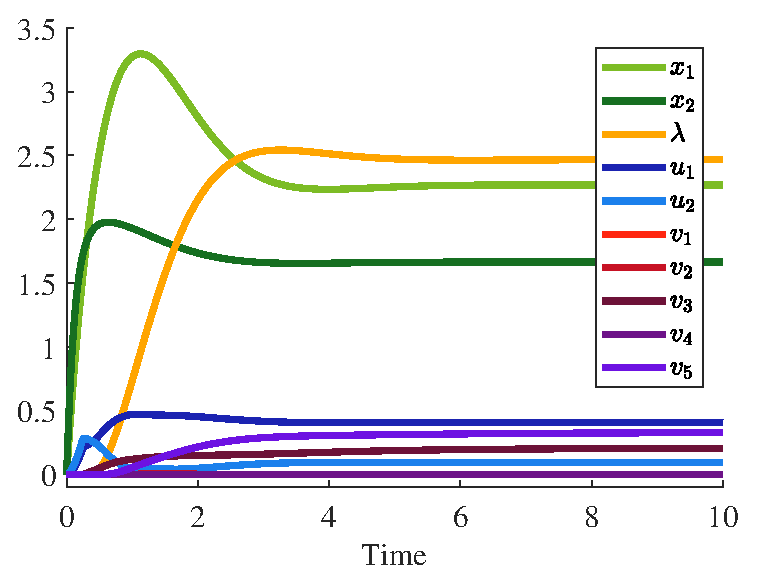
\includegraphics[scale=0.55]{trajectories_intersection.eps}
\vspace{-1.5mm}
\caption{Trajectories of ${\cal RO}$ dynamics for the robust QP problem with intersection of ellipsoids uncertainty set in Example A.}
\label{trajectories_norm_intersection}
\end{center}
\end{figure}
\begin{figure}
\begin{center}
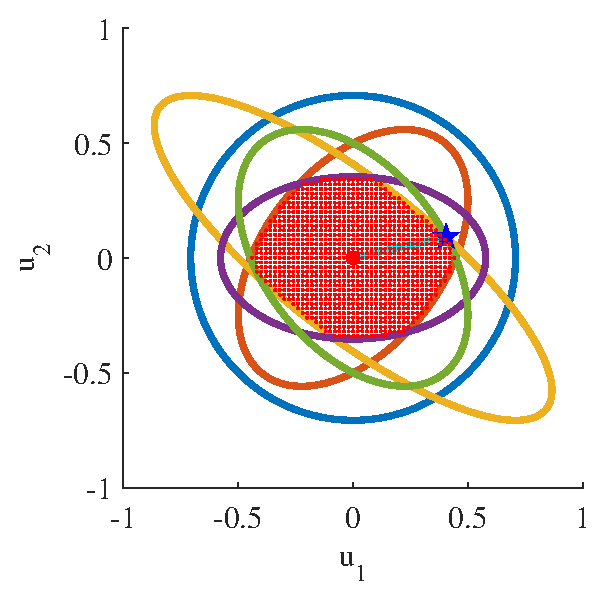
\includegraphics[scale=0.55]{ellipsoids}
\vspace{-1.5mm}
\caption{Uncertainty set for the Example A plotted in $u_
2$-$u_1$ space. The big red point at the origin represents the initial point of $u$ in ${\cal RO}$ dynamics and the blue star depicts the optimal value of $u$ on the intersection of two ellipsoids derived by our method. The small red grid points are the $1115$ sampled points from the uncertainty set in randomized scenario method \cite{calafiore2004} to compare with our method.}
\vspace{-8mm}
\label{ellipsoids}
\end{center}
\end{figure}

\subsection{Robust Nonlinear Optimization with no RC}\label{norc.sec}

Consider the following robust nonlinear optimization problem
\begin{align} \label{ro_simulation_3}
&\min_{x \in \mathbf{R}^2} \;f(x):=\frac{1}{2}(x_1-1)^2+\frac{1}{2}(x_2-2)^2\\
&\;\;\;\text{s.t.}\;\;\max_{u\in {\cal U}} u^\top \left[\begin{array}{ccl}e^{x_1^2}\\e^{x_2^2} \end{array}\right] \leq b\;,\;\nonumber
\end{align}
where $x \in \mathbf{R}^2$, and $u=[u_1, u_2]^\top \in \mathbf{R}^2$, for which, the strictly convex uncertainty set is described by
\begin{align} \label{uncertasinty_example3}
{\cal U}:=\{u \in \mathbb{R}^{2}:e^{u_j^2}+u_j e^{\frac{1}{u_j}} \leq \rho_j\;,\; j=1,2\}\;.
\end{align}
As stated in \cite{bental20152} and \cite{gorissen20152}, there is no closed-form convex conjugate for the constraint (convex in $x$) in (\ref{ro_simulation_3}) and no closed-form conjugate for the convex uncertainty set in (\ref{uncertasinty_example3}). This is the third case in \cite[~Table 1]{gorissen20152}, for which there is no known method for obtaining RC. However, by writing the Lagrangian function as
\begin{align*}
{\cal L}=&\frac{1}{2}(x_1-1)^2+\frac{1}{2}(x_2-2)^2\\
&+\lambda \Big(u^\top \Big[\begin{array}{ccl}e^{x_1^2}\\e^{x_2^2} \end{array}\Big]-b-v^\top \Big[\begin{array}{cc} e^{u_1^2}+u_1 e^{\frac{1}{u_1}}-\rho_1 \\ e^{u_2^2}+u_2 e^{\frac{1}{u_2}}-\rho_2 \end{array}\Big]\Big)\;,
\end{align*}
where $h_j(u_j)=e^{u_j^2}+u_j e^{\frac{1}{u_j}}-\rho_j$ for $j=1,2$ as defined in the previous example, we can form the ${\cal RO}$ dynamics for the RNO problem (\ref{ro_simulation_3}) as
\begin{align*}
&\dot x=-\Big[\begin{array}{ccl} x_1-1 \\ x_2-2 \end{array}\Big]-\hat{\lambda}\; \Big[\begin{array}{cc} 2 x_1 e^{x_1^2} & 0 \\ 0 & 2 x_2 e^{x_2^2}\end{array}\Big]u \nonumber\;,\\
&\dot {\hat{\lambda}} = \Big[u^\top \Big[\begin{array}{cc} e^{x_1^2}\\ e^{x_2^2}\end{array}\Big]-b- \sum_{j=1}^2 \big(v_j(e^{u_j^2}+u_j e^{\frac{1}{u_j}}-\rho_j)\big)\Big]_{\hat{\lambda}}^{\varepsilon+}\nonumber\;,\\
&\dot u=\Big[\begin{array}{cc} e^{x_1^2}\\ e^{x_2^2}\end{array}\Big]- \sum_{j=1}^2(2u_j e^{u_j^2}+e^{\frac{1}{u_j}}-\frac{1}{u_j} e^{\frac{1}{u_j}}) v_j\nonumber\;,\\
&\dot v=\Big[\hat{\lambda}\; \Big[\begin{array}{cc} e^{u_1^2}+u_1 e^{\frac{1}{u_1}}-\rho_1 \\ e^{u_2^2}+u_2 e^{\frac{1}{u_2}}-\rho_2 \end{array}\Big] \Big]_{v}^+\nonumber\;,
\end{align*}
according to ${\cal RO}$ dynamics (\ref{pd_dynamics_0}) where $\hat{\lambda}=\lambda+\varepsilon$. Similarly to the previous example, we can set $\varepsilon$ to zero according to Remark \ref{active_inactive_constraint_rem} as the constraint is active. Fig. \ref{trajectories_nonlinear_exp_no_RC} shows the trajectory plot for $\rho_1=10$, $\rho_2=20$, and all the states initialized at $1$. The robust optimal solution is $[0.5271, 0.7916]$ and the optimal cost value is $0.8419$. We observe that the optimal value for $u$, which is $[1.4020, 1.6824]$ lies on the boundary of the uncertainty set. For positive values of $\varepsilon$, the trajectory and convergence value of $\lambda$ may change, but the solution $x$ remains the same as the constraint is active.

Applying the sampling method in \cite{calafiore2004} with $168$ sampled points in the grid $0.2 \leq u_1 \leq 2$ and $0.2 \leq u_2 \leq 2$ within the uncertainty sets, and solving the many-constrained deterministic problem, the approximate robust optimal solution will be $[0.5376, 0.8193]$, and the approximate optimal cost value is $0.8039$. We again observe that our solution is more exact with a larger cost function value. It is worth mentioning that the solution will be closer to ours by taking more samples in the randomized scenario approach with the cost of adding more constraints to the optimization problem\footnote{For this example, the running time of the sampling scenario method with CVX is more than $200$ times the running time for the ${\cal RO}$ dynamics method.
Furthermore, the sampling method gives less accurate results.}. The reader may imagine how inefficient this approach is when the main $\cal{RO}$ problem has many constraints. The robust counterpart method in \cite{bental2009} nor the one in \cite[~Table 1]{gorissen20152} cannot find the solution as there is no closed-form convex conjugate available for this complicated example. However, the ${\cal RO}$ dynamics easily finds the robust optimal solution.
\begin{figure}
\begin{center}
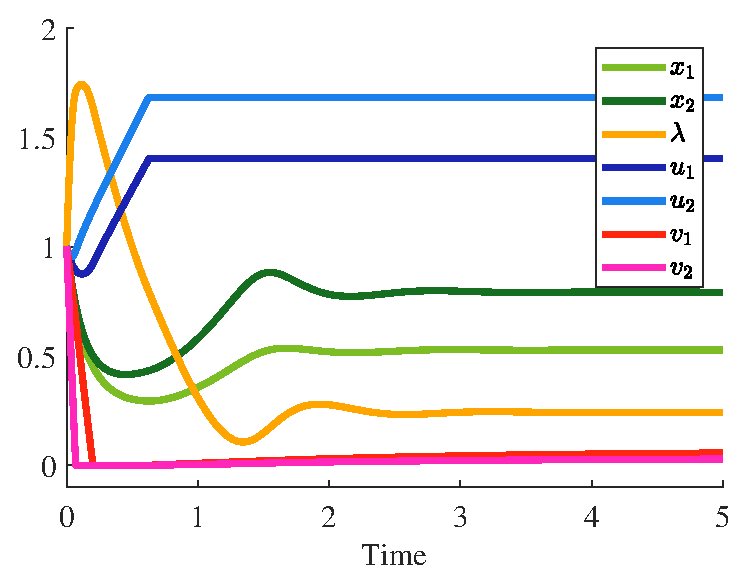
\includegraphics[scale=0.55]{trajectories_nonlinear_exp_no_RC.eps}
\caption{Trajectory of the ${\cal RO}$ dynamics for the robust nonlinear optimization problem (\ref{ro_simulation_3}) in Example B.}
\label{trajectories_nonlinear_exp_no_RC}
\end{center}
\end{figure}

\subsection{Robust Dynamic Location Problem}
We now consider the optimal cooperative and robust self-placement of autonomous vehicles, modeled as first-order kinematic points, to monitor multiple targets (initially assumed static). This is a dynamic generalization of a classical facility location problem \cite{farahani2009} and here we provide a solution to the robust formulation of this problem using ${\cal RO}$ dynamics. The optimization problem is described by an undirected graph with $N$ nodes and a set of edges ${\mathbb E}$. Among these nodes, the first $N_1$ nodes represent the fixed positions of the targets (also referred to as anchors), while the remaining $N_2 = N - N_1$ nodes represent the mobile agents. Each node $x_i\in \mathbb{R}^2$ denotes the location of an anchor or an agent. The anchors $x_1,\cdots,x_{N_1}$ have fixed positions and the agents $x_{N_1+1},\cdots,x_{N}$ are mobile and can adjust their positions. The problem is to find the locations of the sensor nodes $x_{N_1+1},\cdots, x_N$ to minimize the following cost
\begin{align*}
g(x_1,..,x_{N_1})=\min_{x_{N_1+1},\cdots,x_N} \sum_{(i,j)\in {\mathbb E}}
f_{ij}(x_i, x_j)\;,
\end{align*}
which is the sum of some measure of "length" for each link. This problem and its generalizations have many applications \cite{boyd2004}, and can be solved efficiently and in a distributed fashion in continuous time \cite{wang2011}. Leaving the sensor nodes (agents) mobile and capable of computation in distributed mode, we obtain a distributed dynamical version \emph{real-time} of the optimal placement. The sensor nodes, through local interactions, cooperate to find and move toward their globally optimal locations autonomously.

The problem can also be under a set of constraints for the position of agents $x_{N_1+1},\cdots,x_{N_1}$ to be in a specified convex set. Specifically, we consider the following robust location and placement problem
\begin{align*}
    &\min_{x_{N_1+1},\cdots,x_N} \sum_{(i,j)\in {\mathbb E}} \frac{1}{2}\; w_{ij} \parallel x_i - x_j \parallel_2^2\\
    &\;\;\text{s.t.}\;\;\underset{u_i\in {\cal U}_i}{\max} (a_i+P_i u_i)^\top x_i \leq b_i, \; i={N_1+1},\cdots,N\;,
\end{align*}
where the uncertainty $u_i$ lies in ${\cal U}_i = \parallel u_i \parallel_2^2\; \leq \rho_i^2$ and $x_{N_1}+1,\cdots,x_{N}$ are moving agents. The ${\cal RO}$ dynamics for this problem can be derived as follows for $i=N_1+1,\cdots,N$
\begin{align*}
\left\{
\begin{array}{cl}
\vspace{2mm}
&\dot{x}_i=\sum_j w_{ij} (x_i-x_j)-\hat \lambda_i \; (a_i+P_i u_i)\\
\vspace{2mm}
&\dot{\hat \lambda}_i=[(a_i+u_i P_i)^\top x_i-P_i u_i^\top c_i-b_i-v_i\; {\cal U}_i]_{\hat \lambda_i}^{\varepsilon+}\\
\vspace{2mm}
&\dot{u}_i=P_i^\top (x_i-c_i)-2v_i u_i\\
\vspace{2mm}
&\dot{v}_i=[\hat \lambda_i\; {\cal U}_i]
\vspace{2mm}
\end{array}\right..
\end{align*}
Note that this problem is naturally distributed and our dynamics reflects the distributed structure. We consider the setup shown in Figure \ref{fig_points} with five anchors and four agents. The figure also shows the (fixed) interconnection graph among all the elements of the problem. In this academic example, we consider the presence of a linear constraint defining the half-space where the agents can be. The constraint is simply
\begin{align*}
{\bf 1}'x_i\leq 2.5, \;\; i=N_1+1,\cdots,N\;,
\end{align*}
for all the agents.
In addition, we would like the agents to find robust locations based on the uncertainty on the nominal slope $45^o$ of the nominal constraint. Namely
\begin{align*}
{\bf 1}'x_i+u_iP'x_i\leq 2.5,\;\; i=N_1+1,\cdots,N\;,
\end{align*}
where $P'=\begin{bmatrix}1&-1\end{bmatrix}$ and $\|u_i\|_2^2\leq \rho^2$. For example, when $\rho=1$, the constraint can be any line passing through $x'=(1.25,\,1.25)$, including the horizontal and vertical ones. Figure \ref{fig_points} also shows the nominal linear constraint. The location of the shown agents is the optimal robust one w.r.t. the constraint being perturbed by the uncertainty $u_i$ with $\|u_i\|_2^2\leq 0.1$.

First, agents start at their initial locations at the origin (white circle), and their paths converge to the optimal robust location for $\rho^2=0.1$. Such locations are indicated by full-colored circles. We see that agents $1$ and $4$ (blue and green) are on the boundary of the robust feasible set identifiable with the larger sector in the figure. The uncertain constraint is not active for the other agents. However, their optimal location is indirectly influenced by the robust constraint active in agents $1$ and $4$ as all agents and anchors are interconnected.

In the next phase of the simulation, we rotate the location of the anchors clockwise at constant speed. Although agents only react to their local neighbors (agents/anchors), the interconnected dynamical system shows the ability to globally track the coordinated motion of the anchors within the robust feasible set. It is interesting to notice that the boundary of the feasible set is not defined a priori or hard-coded in the simulation, but it emerges from the interactions built in the dynamical system. Finally, after some time, the uncertainty changes and increases with size $\rho^2=1$ at time $t=300$. This implies that no location should be feasible above the horizontal line passing through $(1.25,1.25)$ and on the right of the vertical line passing through the same point. The location of the agents when the uncertainty changes is indicated by black empty circles. We note that, when the uncertainty changes, the nodes $1$, $2$, and $3$ are located outside the new robust feasible set and, with a transient correction, move inside the robust SW quadrant for the rest of the time.

This example showcases the ability of the dynamical system to track changes online and adapt to uncertainty changes over time. We have obtained the behavior shown by appropriate scaling of the various differential equations involved. Note that the convergence is not affected by positive scaling of the differential equations. A relatively larger scaling on the dual variables in charge of the constraints makes the system response more reactive toward feasibility and more sensitive toward uncertainty changes. We leave to future research the systematic design of the optimization system for the desired real-time behavior.

\begin{figure}
\begin{center}
\includegraphics[scale=0.26]{simulation_figure_finalv3.png}
\vspace{-1.5mm}
\caption{Locations of agents and anchors, interactions between agents and anchors, and the nominal linear constraint in Example C.}
\label{fig_points}
\end{center}
\end{figure}

\section{Conclusions}\label{section_conclusions}
We proposed a continuous-time dynamical system, ${\cal RO}$ dynamics, to solve robust optimization problems. This approach can solve convex-concave ${\cal RO}$ problems in a decentralized manner without requiring specific model knowledge. This approach offers an advantage over existing methods, which are based on robust counterpart and random sampling particularly for problems with large scales, complex constraint and uncertainty sets, real-time adaptation requirements or unknown dynamics. The implementation capability of ${\cal RO}$ dynamics, elaborated in this paper, opens new avenues for robustifying large-scale optimization problems in Machine Learning and Deep Learning against uncertainties, perturbations, and adversarial attacks, while further research is needed to analyze the computational cost and rigorously characterize the convergence rate of ${\cal RO}$ dynamics.
\section{Appendix} \label{section_appendix}

\subsection{Lemma \ref{saddle.lem} [Saddle property]}
Essentially, we want to show that
\begin{align*}
{\cal L}(x^\star,\lambda,u,v^\star)\leq \mu \leq {\cal L}(x,\lambda^\star,u^\star,v)\;.
\end{align*}
Under Assumption \ref{assume_feasible}, an optimal solution $x^\star$ exists and based on Assumption \ref{assume1}, this optimal solution is unique as $f_0(x,u_0)$ is strictly convex in $x$ for any $u_0 \in{\cal U}_0$. Consider any optimal solution $(x^\star,\lambda^\star,u^\star,v^\star)$ for ${\cal RO}$ problem (\ref{dual.eq}).

\noindent
For each of the lower level optimizations, let
\begin{align*}
\eta_i=\max_{u_i\in {\cal U}_i}f_i(x^\star,u_i)=f_i(x^\star,u_i^\star)=
\tilde{\cal L}_i(x^\star,u_i^\star,v_i^\star),\; i_{[N]}\;.
\end{align*}
From the corresponding saddle property, it follows that for all $u_i$, $i_{[N]}$,
\begin{equation}\label{xxlb.eq}
f_i(x^\star,u_i)-(v_i^\star)^\top h_i(u_i)\leq \eta_i\;.
\end{equation}
From the upper level saddle property, for all $\lambda_i\geq 0$, $i^+_{[N]}$,
\begin{align*}
\eta_0+\sum_i(c_i+\lambda_i)\eta_i\leq f_0(x^\star,u_0^\star)+\sum_{i=1}^N(c_i+\lambda_i^\star)\eta_i=\mu\;.
\end{align*}
Substituting the lower bound on $\eta_i$, (\ref{xxlb.eq}), in the left hand side, it follows that for all $u_i, i_{[N]}$ and $\lambda_i\geq 0, i^+_{[N]}$,
\begin{align*}
&{\cal L}(x^\star,\lambda,u,v^\star)\\
= &f_0(x^\star,u_0)-(v_0^\star)^\top h_0(u_0)\\
& +\sum_{i=1}^
N(c_i+\lambda_i)(f_i(x^\star,u_i)-(v_i^\star)^\top h_i(u_i))\\
\leq &\;\mu\;,
\end{align*}
where we have used $c_i+\lambda_i\geq 0$. We next use lower saddle property in the other direction, namely, for all $v_i\geq 0$,
\begin{align*}
\eta_i=f_i(x^\star,u_i^\star)=f_i(x^\star,u_i^\star)-(v_i^\star)^\top h_i(u_i^\star)\\
\leq f_i(x^\star,u_i^\star)-(v_i)^\top h_i(u_i^\star)\;,
\end{align*}
which implies that for all $v_i\geq 0$, $-v_i^\top h(u^\star)\geq 0$, $i_{[N]}$.\\
Using this property and the fact that $(c_i+\lambda_i^\star)\geq 0$, it follows that for all $v_i\geq 0$, $i^+_{[N]}$,
\begin{equation}\label{xxub.eq}
-(v_0)^\top h_0(u_0^\star)-\sum_{i=1}^N(c_i+\lambda_i^\star)(v_i)^\top h_i(u_i^\star)\geq 0\;.
\end{equation}

\noindent
The upper level saddle property implies
\begin{align*}
\mu\leq f_0(x,u_0^\star)+\sum_{i=1}^N(c_i+\lambda_i^\star)f_i(x,u_i^\star)
\end{align*}
for all $x$. Combining this with (\ref{xxub.eq}), we obtain
\begin{align*}
\mu&\leq f_0(x,u_0^\star)-(v_0)^\top h_0(u_0^\star)\\
&+\sum_{i=1}^N(c_i+\lambda_i^\star)(f_i(x,u_i^\star)-(v)^\top h_i(u_i^\star))\\
&={\cal L}(x,\lambda^\star,u^\star,v)
\end{align*}
for all $x$ and $v_i\geq 0, i_{[N]}$.
\qed

\subsection{${\cal RO}$ dynamics solutions properties}\label{existence.sec}
${\cal RO}$ dynamics (\ref{pd_dynamics}) can be viewed as switched dynamical system with a discontinuous right-hand side. The conditions guaranteeing the existence and uniqueness of the solution and continuity w.r.t. initial conditions, for a general discontinuous dynamical system are provided in \cite[Theorem~2.5]{nagurney2012projected}. In this section, we show that our ${\cal RO}$ dynamics (\ref{pd_dynamics}) satisfies the refined conditions presented in \cite{cherukuri2016}.

To prove the existence and uniqueness of solutions for (\ref{pd_dynamics}), and also the continuity of solutions w.r.t. the initial conditions, there are two main steps. The first step is showing that ${\cal RO}$ dynamics is a particular case of projected dynamical systems. The second step requires ${\cal RO}$ dynamics (\ref{pd_dynamics}) satisfying the monotonicity property, which is our main result.

\begin{definition} \label{projection_operator} (Projection operator)
If ${\cal K}$ is a closed convex set, for any point $\bar y \in \mathbb R^q$, the point projection of $\bar y$ on the set ${\cal K}$ can be written as
\begin{align*}
\text{proj}_{\cal K}(\bar y)=\text{argmin}_{y \in {\cal K}} \parallel y-\bar y \parallel\;.
\end{align*}
For $\bar y \in \mathbb R^n$ and $y \in {\cal K}$, vector projection of $\bar y$ at $y$ w.r.t. ${\cal K}$ is
\begin{align}
\label{projection_operator}
\Pi_{\cal K}(y,\bar y) = \text{lim}_{\delta \rightarrow 0^+} \frac{\text{proj}_{\cal K}(y+\delta \bar y)-y}{\delta}\;.
\end{align}
\end{definition}

Note that the map $\text{proj}_{\cal K}$ is Lipschitz on $\mathbb R^q$ with constant $L=1$ \cite[Proposition~2.4.1]{clarke1983}.

\begin{definition} \label{projected_dynamical_system} [Projected dynamical system \cite{nagurney1996}]
Considering a differential equation $\dot y=F(y)$ with $F:\mathbb R^q \rightarrow \mathbb R^q$, the associated projected dynamical system is defined as
\begin{align}
\label{projected_dynamics}
\dot y = \Pi_{\cal K}(y,F(y)),\; y(0) \in {\cal K}\;.
\end{align}
\end{definition}

\begin{lemma} \label{projected} (${\cal RO}$ dynamics as a projected dynamics)
${\cal RO}$ dynamics (\ref{pd_dynamics}) can be written as a projected dynamical system according to Definition \ref{projected_dynamical_system}.
\end{lemma}
\begin{proof}
The proof of Lemma \ref{projected} follows along the lines of the construction outlined in \cite{cherukuri2016}. Details omitted. \qed\\
\end{proof}

\begin{proposition} \label{proposition_projected}
If $F$ in the projected dynamical system (\ref{projected_dynamics}) is Lipschitz on ${\cal K}$, we have the following existence, uniqueness, and continuity w.r.t. the initial condition results for the solutions of the projected dynamics (\ref{projected_dynamics}):
\begin{enumerate}
\item For any $y_{0} \in {\cal K}$, there exists a unique solution $t \rightarrow y(t)$ of the projected system (\ref{projected_dynamics}) with $y(0)=y_{0}$ in $[0,\infty)$.
\item Consider a sequence of points $\{y_{k}\}_{k=1}^\infty \subset {\mathcal K}$ with $lim_{k \rightarrow \infty}=y$. Then, the sequence of solutions $\{t \rightarrow \gamma_k(t)\}_{k=1}^\infty$ of the projected dynamics (\ref{projected_dynamics}) with $\gamma_k(0)=y_k$ for all $k$, converges to the solution $t \rightarrow \gamma(t)$ of (\ref{projected_dynamics}) with $\gamma(0)=y$ uniformly on every compact set of $[0,\infty)$.
\end{enumerate}
\end{proposition}
The ability to write ${\cal RO}$ dynamics (\ref{pd_dynamics}) as a projected dynamical system along with the monotonicity property is used in the proof of the existence, uniqueness and continuity of the solutions of the set ${\mathbb S}$.

\begin{lemma} \label{uniq_exis}
(Existence, uniqueness and continuity of solutions)
$\gamma:[0,T) \rightarrow {\mathbb S}$ is defined as a Caratheodory solution of ${\cal Z}^{\cal RO}$ in the interval $[0,T)$ if $\gamma$ is absolutely continuous on $[0,T)$ and satisfies $\dot \gamma(t)={\cal Z}^{\cal RO} (\gamma(t))$ almost everywhere in $[0,T)$.
Under Assumptions \ref{assume1} and \ref{assume_feasible}, and starting from any point $z\in \mathbb S$, a unique solution to ${\cal RO}$ dynamics (\ref{pd_dynamics}) exists and remains in $\mathbb S \cap V^{-1}(\leq V(z))$. Also, if a sequence of points $\{z_k\}_{k=1}^\infty \subset {\mathbb S}$ converges to $z$ as $k \rightarrow \infty$, the sequence of solutions $\{t \rightarrow \gamma_k(t)\}_{k=1}^\infty$ of ${\cal Z}^{\cal RO}$ starting at these points (that is, $\gamma_k(0)=z_k$ for all $k$) converge uniformly to the solution $t \rightarrow \gamma(t)$ on every compact set of $[0,\infty)$.
\end{lemma}
The proof of this lemma follows closely along the lines of proof for the existence and uniqueness of solution for the primal-dual dynamical system from \cite[Lemma~4.3]{cherukuri2016}.

\subsection{Theorem \ref{RO_ROperturbed}}

Based on the optimal solution $x^\star$ for ${\cal RO}$ problem,
\begin{align*}
\mu=\min_{{\cal F}_i(x)\leq  0} {\cal F}_0(x)\;,\; \mu={\cal F}_0(x^\star)\;.
\end{align*}
As the cost function of $\mu_\varepsilon$ is smaller than or equal to that of ${\cal RO}$ and the feasible sets of the two problems are equal,
\begin{equation}\label{ub.eq}
 \mu_\varepsilon-\mu\leq 0\;.
\end{equation}
Since $x^\star$ minimizes ${\cal F}_0(x)$ over the constraint set, $\mu={\cal F}_0(x^\star)\leq {\cal F}_0(x_\varepsilon^\star)$.
Adding and subtracting $\varepsilon\sum_{i=1}^n{\cal F}_i(x^\star_\varepsilon)$
in the RHS and using (\ref{ub.eq}) yields $\varepsilon \sum_{i=1}^N{\cal F}_{i}(x_\varepsilon^\star)\leq
\mu_\varepsilon-\mu\leq 0$\;.

Following a similar argument as before by comparing $\mu(\varepsilon_0)$ and $\mu_\varepsilon$ for $\varepsilon_0\geq \varepsilon$, we now let
\begin{align*}
&\mu_\varepsilon=\tilde{{\cal F}}_0(x^\star_\varepsilon)={\cal F}_0(x^\star_\varepsilon)+\varepsilon\sum_{i=1}^N{\cal F}_i(x^\star_\varepsilon)\;,\\
&\mu(\varepsilon_0)=\tilde{{\cal F}}_0(x^\star_{\varepsilon_0})+\delta\sum_{i=1}^N{\cal F}_i(x^\star_{\varepsilon_0})\;,
\end{align*}
where $\delta=\varepsilon_0-\varepsilon$. Then, $\mu_\varepsilon\geq \mu(\varepsilon_0)$\;,
but because $x_\varepsilon^\star$ is optimal for $\mu_\varepsilon$\;, we have
$\tilde{{\cal F}}_0(x^\star_\varepsilon)\leq \tilde{{\cal F}}_0(x^\star_{\varepsilon_0})$.
As $x^\star_\varepsilon$ is feasible for $\mu(\varepsilon_0)$, \begin{align*}
\tilde{{\cal F}}_0(x^\star_{\varepsilon_0})+\delta\sum_{i=1}^N{\cal F}_i(x^\star_{\varepsilon_0})=\mu(\varepsilon_0)\leq \tilde{{\cal F}}_0(x^\star_{\varepsilon})+\delta\sum_{i=1}^N{\cal F}_i(x^\star_{\varepsilon})\;.
\end{align*}
Combining the two inequalities,
\begin{align*}
\delta\sum_{i=1}^N{\cal F}_i(x^\star_{\varepsilon_0})-\delta\sum_{i=1}^N{\cal F}_i(x^\star_{\varepsilon})\leq \tilde{{\cal F}}_0(x^\star_{\varepsilon})-\tilde{{\cal F}}_0(x^\star_{\varepsilon_0})\leq 0\;,
\end{align*}
which implies that $\sum_{i=1}^N{\cal F}_i(x^\star_{\varepsilon_0})\leq \sum_{i=1}^N{\cal F}_i(x^\star_{\varepsilon})$. Thus,
\begin{equation}\label{limi.eq}
\varepsilon\sum_{i=1}^N{\cal F}_{i}(x_{\varepsilon_0}^\star)\leq
\varepsilon\sum_{i=1}^N{\cal F}_{i}(x_{\varepsilon}^\star)\leq
\mu_\varepsilon-\mu \leq 0\;.
\end{equation}
Since $\sum_{i=1}^N{\cal F}_{i}(x_{\varepsilon_0}^\star)=\frac{\mu(\varepsilon_0)-{\cal F}_0(x^\star_{\varepsilon_0})}{\varepsilon_0}$ is bounded, we have
\begin{equation}\label{limi2.eq}
\varepsilon\sum_{i=1}^N{\cal F}_{i}(x_{\varepsilon_0}^\star)\leq
\mu_\varepsilon-\mu\leq 0\;,
\end{equation}
which means that $\mu_\varepsilon$ converges to $\mu$ as $\varepsilon\to 0$.

To prove the second part of the theorem, that is, $x^\star_\varepsilon \to x^\star$ as $\varepsilon \to 0$, consider any sequence $\{\varepsilon_n\}$ converging to $0$. Let $\{x^\star_{n}\}$ be the corresponding sequence of optimal solutions for $\mu(\varepsilon_n)$.

As ${\cal C}$ is compact and the same for both perturbed and original problem, $x^\star_{n}\in {\cal C}$ is bounded.  Therefore, there exists a convergent sub-sequence $x_{n_t}^\star$ that converges to, say, $\hat{x}\in {\cal C}$, as $\varepsilon_{n_t} \to 0$, since ${\cal C}$ is closed by assumption.

This implies that
${\cal F}_0(x_{n_t}^\star) \to {\cal F}_0(\hat{x})\;,$ since ${\cal F}_0(x)$ is continuous.
Because $\hat{x}$ is feasible, ${\cal F}_0(\hat{x})\geq \mu$.
However,  ${\cal F}_0(\hat{x})>\mu$ is impossible since
$
\mu(\varepsilon_{n_t})\to \mu
$,
from the first part of the proof, and $\displaystyle\mu(\varepsilon_{n_t})={\cal F}_0(x^\star_{n_t})+\varepsilon_{n_t}\sum_{i=1}^N{\cal F}_{i}(x_{n_t}^\star)\to {\cal F}_0(\hat{x})$, since from (\ref{limi.eq}) and (\ref{limi2.eq}), $\displaystyle\lim_{\varepsilon_{n_t}\to 0}
\varepsilon_{n_t}\sum_{i=1}^N{\cal F}_{i}(x_{\varepsilon_{n_t}})=0$\;.

Therefore, ${\cal F}_0(\hat{x})=\mu={\cal F}_0(x^\star)$. Since $f(x)$ is strictly convex, $\hat{x}=x^\star$. Since every convergent sub-sequence converges to $x^\star$, the whole sequence converges to it. Since the sequence was arbitrary, we have that $x^\star_\varepsilon\to x^\star$ as $\varepsilon\to 0$\;.

\bibliography{2.References}
\bibliographystyle{ieeetr}
\begin{IEEEbiography}
[{\includegraphics[width=1in,height=1.25in,clip,keepaspectratio]{k1.jpg}}]
{Keivan Ebrahimi} received bachelor's and master's degree in electrical engineering from Sharif University of Technology, Tehran, Iran in 2012 and 2014. He is a Ph.D. candidate in electrical and computer engineering at Iowa State University (ISU), Ames, IA, USA. He is currently a principal data scientist at Tarana Wireless in Milpitas, CA, USA. He received the College of Engineering fellowship at Iowa State University in 2015 and has been selected for the Rock Star Spot Award for stellar contribution and performance in View Inc. COVID-SENSE product, May 2020. He filed three patents to the United States Patents and Trademarks Office for “Environmental Adjustment using Artificial Intelligence”, “Identifying and Reducing Health Risks and Tracking Occupancy in a Facility”, and “Immersive Collaboration of Remote Participants via Media Displays”. His research interests include adversarial machine learning and deep learning, computer vision, robust optimization, control theory and dynamical systems.
\end{IEEEbiography}

\begin{IEEEbiography}
[{\includegraphics[width=1in,height=1.25in,clip,keepaspectratio]{elia.pdf}}]
{Prof. Nicola Elia} received the Laurea degree in Electrical Engineering from the Politecnico di Torino, Turin, Italy in 1987 and the Ph.D. degree in Electrical Engineering and Computer Science from the Massachusetts Institute of Technology (MIT), Cambridge, MA, USA in 1996. He is currently the Vincentine-Hermes-Luh Chair Professor of Electrical and Computer Engineering at the University of Minnesota (UMN), Twin Cities, MN, USA. Before joining UMN in 2018, and since 1999, he was a faculty with the department of Electrical and Computer Engineering at Iowa State University, Ames, IA, USA. He was a Postdoctoral Associate at the Laboratory for Information and Decision Systems at MIT from 1996 to 1999. He was a Control Engineer with the Fiat research Center, Turin, Italy, from 1987 to 1990. Dr. Elia received the NSF Career Award and he is a Fellow of the IEEE. His research interests include computational methods for controller design, communication systems with access to feedback, control with communication constraints, and network distributed systems.
\end{IEEEbiography}

\begin{IEEEbiography}
[{\includegraphics[width=1in,height=1.25in,clip,keepaspectratio]{umesh.jpeg}}]
{Prof. Umesh Vaidya} received the Ph.D. degree in mechanical engineering from the University of California at Santa Barbara, Santa Barbara, CA, in
2004. He was a Research Engineer at the United Technologies Research Center (UTRC), East Hartford, CT, USA. He is currently a professor in the Department of Mechanical Engineering, Clemson University, S.C., USA. Before joining Clemson University in 2019, and since 2006, he was a faculty with the department of Electrical and Computer Engineering at Iowa State University. He is the recipient of 2012 National Science Foundation CAREER award. His current research interests include dynamical systems and control theory.
\end{IEEEbiography}

\newpage

\end{document}